\documentclass[11pt, twoside, openright]{book}

% Match modern PDF version of embedded figures
\pdfminorversion=7

% Page geometry — 8.5x11 with gutter (mirrors In the Studio v12)
\usepackage[
  paperwidth=8.5in,
  paperheight=11in,
  inner=1.375in,
  outer=1.0in,
  top=0.90in,
  bottom=1.0in,
  headheight=14pt,
  headsep=0.2in,
  footskip=0.35in
]{geometry}

% Fonts — Palatino via mathpazo (matches Studio book)
\usepackage[T1]{fontenc}
\usepackage[utf8]{inputenc}
\usepackage{mathpazo}
\linespread{1.15}
\usepackage{microtype}

% Essential packages
\usepackage{graphicx}
\usepackage[table]{xcolor}
\usepackage{booktabs}
\usepackage{tabularx}
\usepackage{longtable}
\usepackage{tcolorbox}
\tcbuselibrary{breakable, skins}
\usepackage{fancyhdr}
\usepackage{titlesec}
\usepackage{tocloft}
\usepackage{enumitem}
\usepackage{csquotes}
\usepackage{textcomp}
\usepackage{amssymb}
\usepackage{amsmath}
\usepackage{gensymb}
\usepackage{float}
\usepackage{placeins}
\usepackage[hidelinks]{hyperref}
\hypersetup{
  pdftitle={Consensus Change Standards: A Legal and Technical Framework for Bitcoin Protocol Governance},
  pdfauthor={Asaf Fulks},
  pdfsubject={Bitcoin Protocol Governance},
  pdfcreator={The Forum Press}
}
\usepackage{bookmark}
\usepackage{emptypage}
\usepackage{eso-pic}  % full-bleed cover image on page i
\usepackage{caption}
\usepackage{needspace}
\usepackage{etoolbox}

% Caption styling
\captionsetup{
  font=small,
  labelfont=bf,
  textfont=it,
  width=0.85\textwidth,
  justification=centering,
  singlelinecheck=off
}

% Colors (mirrors Studio book)
\definecolor{chaptergray}{RGB}{80, 80, 80}
\definecolor{sectioncolor}{RGB}{40, 40, 40}

% Chapter title formatting
\titleformat{\chapter}[display]
  {\normalfont\huge\bfseries\color{chaptergray}}
  {\chaptertitlename\ \thechapter}{20pt}{\Huge}
\titlespacing*{\chapter}{0pt}{-20pt}{30pt}

% Section formatting
\titleformat{\section}
  {\needspace{4\baselineskip}\normalfont\Large\bfseries\color{sectioncolor}}{\thesection}{0.7em}{}
\titlespacing*{\section}{0pt}{18pt}{8pt}

% Subsection formatting
\titleformat{\subsection}
  {\needspace{3\baselineskip}\normalfont\large\bfseries\color{sectioncolor}}{\thesubsection}{0.6em}{}
\titlespacing*{\subsection}{0pt}{14pt}{6pt}

% Header/footer
\pagestyle{fancy}
\fancyhf{}
\fancyhead[LE]{\small\textit{Consensus Change Standards}}
\fancyhead[RO]{\small\textit{\leftmark}}
\fancyfoot[C]{\thepage}
\renewcommand{\headrulewidth}{0.4pt}

% Plain pages (chapter starts)
\fancypagestyle{plain}{
  \fancyhf{}
  \fancyfoot[C]{\thepage}
  \renewcommand{\headrulewidth}{0pt}
}

% List spacing
\setlist[itemize]{nosep, leftmargin=2em, topsep=4pt, parsep=2pt}
\setlist[enumerate]{leftmargin=2em, topsep=4pt, itemsep=6pt, parsep=2pt}

% Paragraph spacing
\setlength{\parindent}{0pt}
\setlength{\parskip}{6pt plus 2pt minus 1pt}

% TOC formatting
\renewcommand{\contentsname}{Contents}
\setlength{\cftchapnumwidth}{2.5em}
\renewcommand{\cftchapaftersnum}{.}

% Prevent widows and orphans
\widowpenalty=10000
\clubpenalty=10000

\emergencystretch=3em
\hyphenation{con-sen-sus block-chain hash-rate}

% Prevent section headings from appearing at bottom of page without content
\pretocmd{\section}{\needspace{4\baselineskip}}{}{}
\pretocmd{\subsection}{\needspace{3\baselineskip}}{}{}

% Float placement
\renewcommand{\topfraction}{0.9}
\renewcommand{\bottomfraction}{0.9}
\renewcommand{\textfraction}{0.07}
\renewcommand{\floatpagefraction}{0.85}
\setcounter{topnumber}{3}
\setcounter{bottomnumber}{2}
\setcounter{totalnumber}{5}

% Tighten spacing around floats
\setlength{\floatsep}{8pt plus 2pt minus 2pt}
\setlength{\textfloatsep}{10pt plus 2pt minus 2pt}
\setlength{\intextsep}{8pt plus 2pt minus 2pt}
\setlength{\abovecaptionskip}{6pt}
\setlength{\belowcaptionskip}{2pt}

\raggedbottom

% Definition term helper for the glossary
\newcommand{\defterm}[1]{\textbf{#1}}

% Lettered-subitem helper for A./B./C. style standards within a section
\newcommand{\reqitem}[2]{\medskip\noindent\textbf{#1\ #2}\quad\ignorespaces}

% Section reference shorthand
\newcommand{\sect}[1]{\S#1}

% "In Brief" sidebar — light-gray tcolorbox for end-of-chapter recaps.
% Unbreakable: combined with \needspace before each box, this keeps boxes whole.
\newtcolorbox{plainenglish}{
  enhanced,
  colback=gray!5,
  colframe=gray!45,
  boxrule=0.4pt,
  arc=2.5pt,
  left=12pt,
  right=12pt,
  top=8pt,
  bottom=8pt,
  before skip=14pt,
  after skip=14pt,
  fontupper=\small,
  before upper={\setlength{\parskip}{6pt plus 2pt minus 1pt}\setlength{\parindent}{0pt}},
}
\newcommand{\peheader}[1]{{\itshape\bfseries #1}\par\vspace{4pt}}

\begin{document}

\frontmatter

% =========================================================================
% COVER (full-bleed page i)
% =========================================================================
\AddToShipoutPicture*{%
  \put(0,0){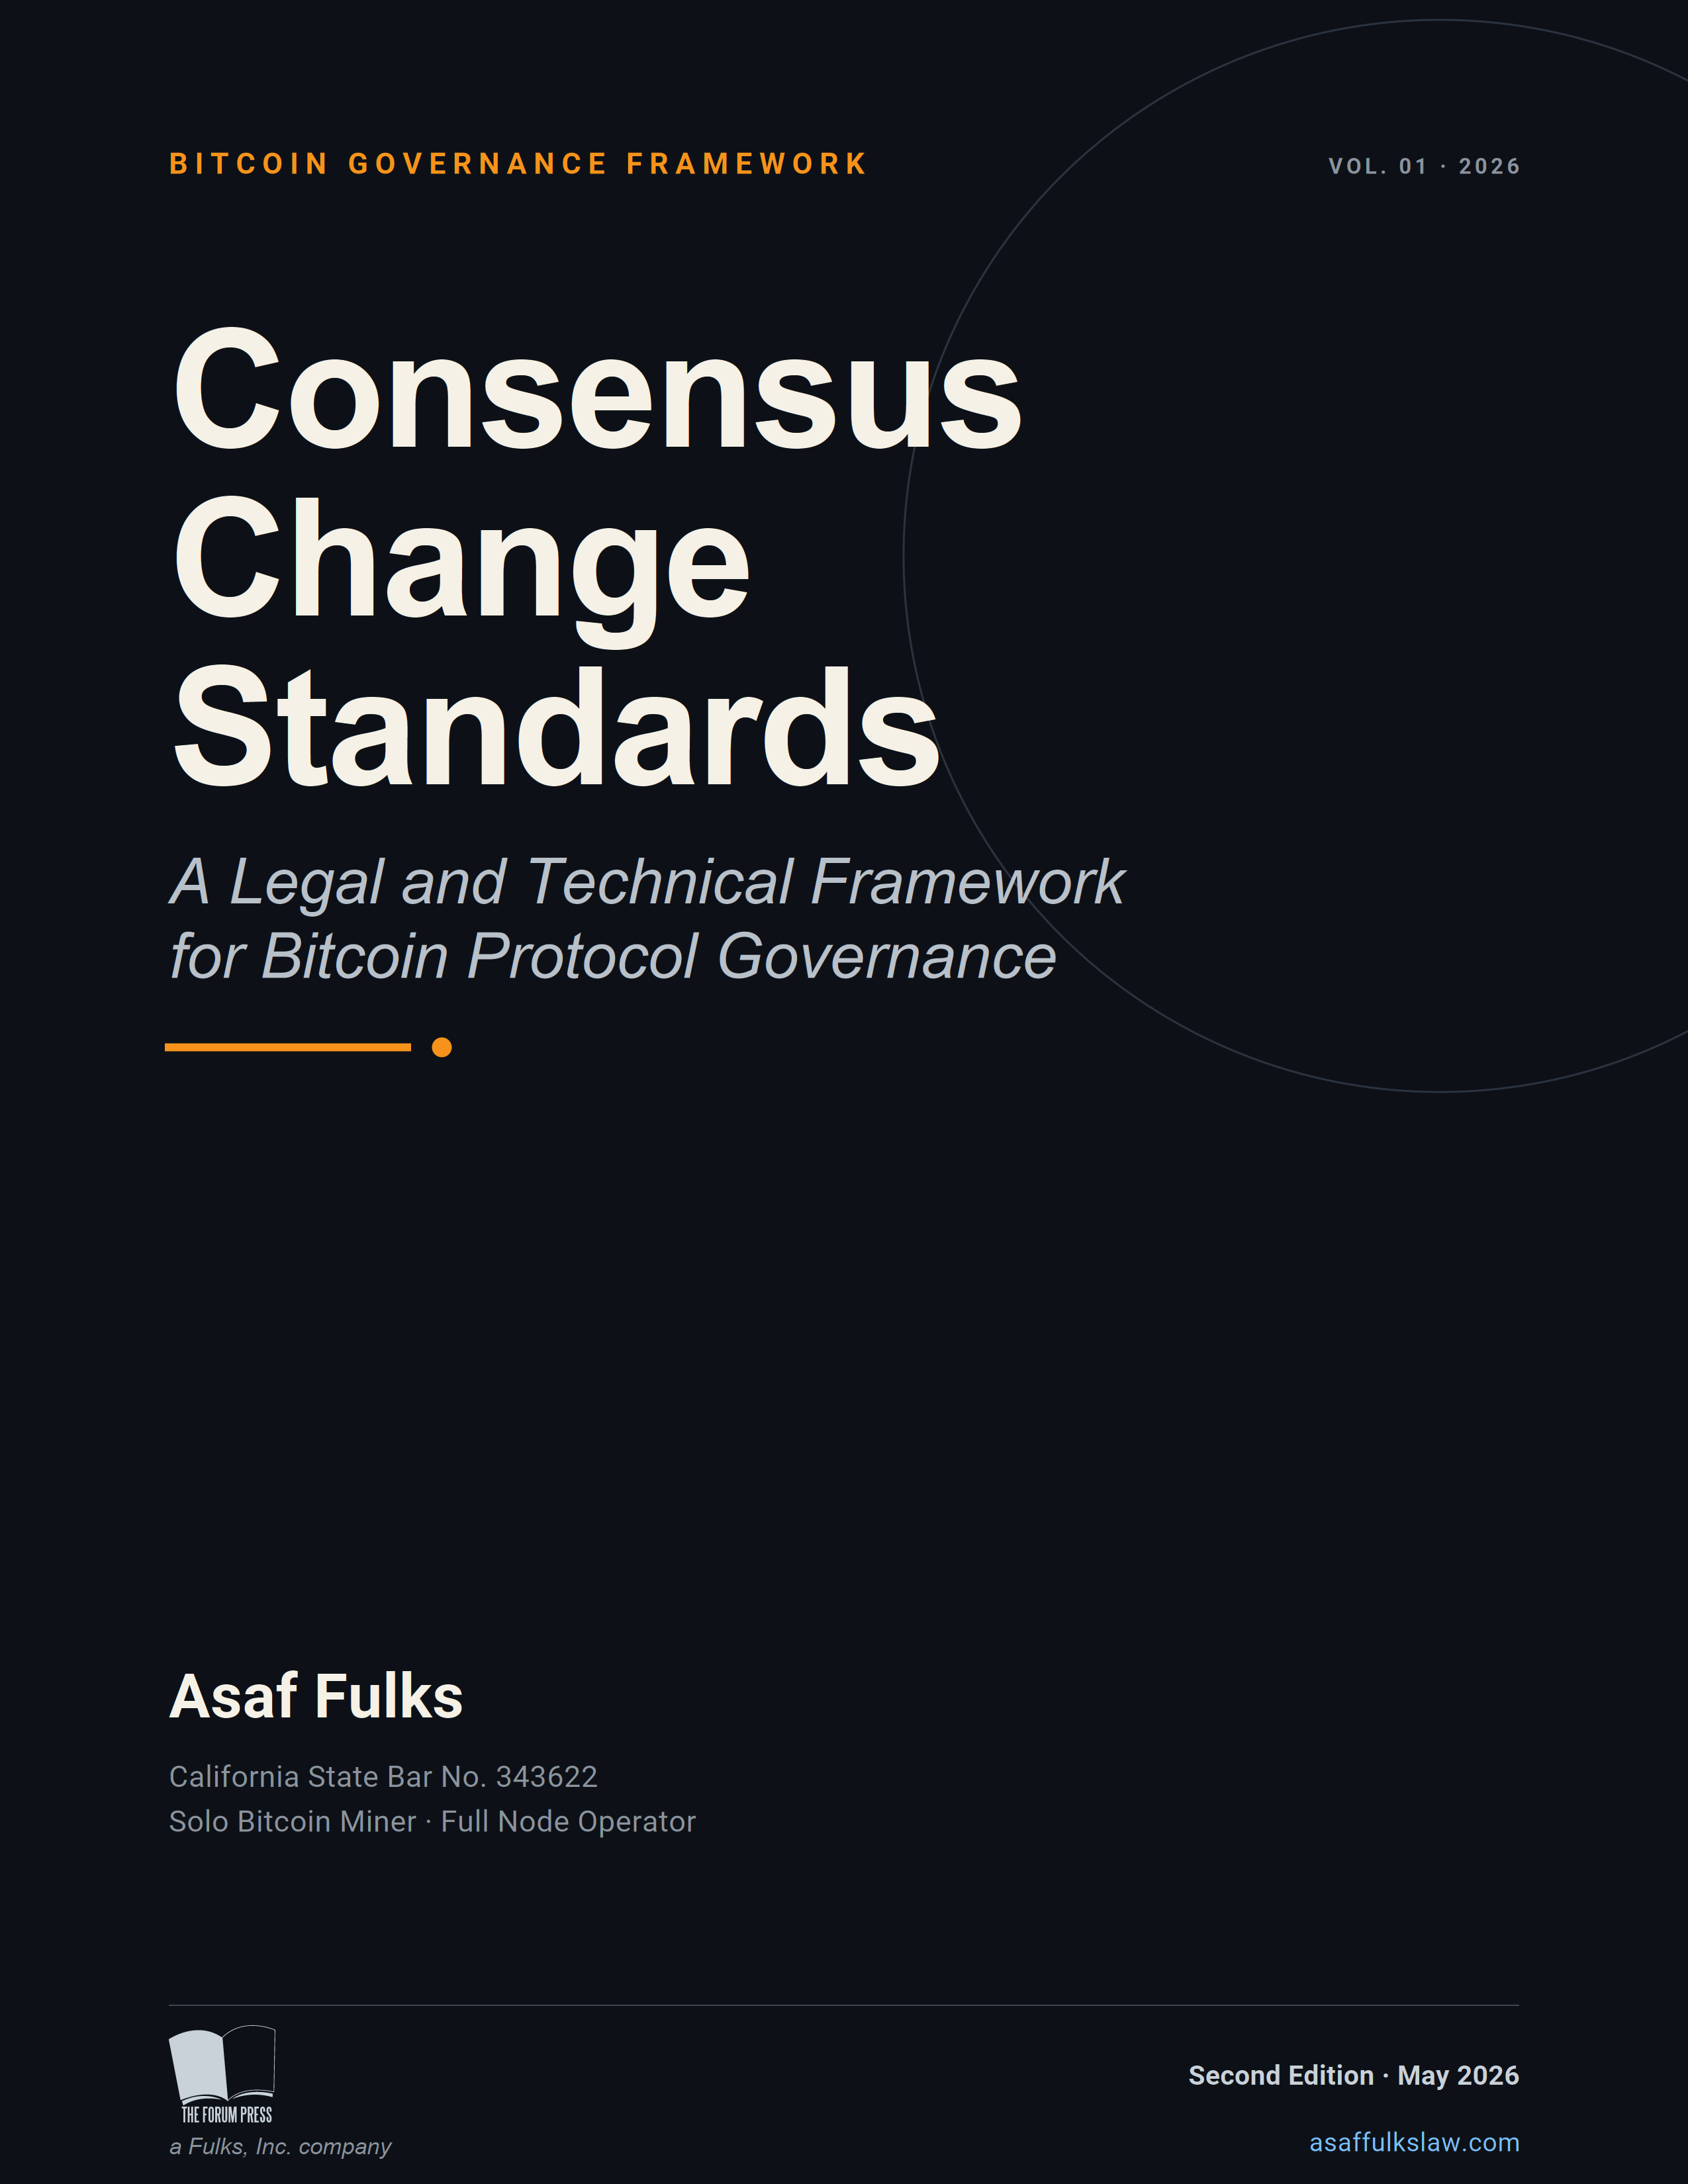
\includegraphics[width=\paperwidth,height=\paperheight]{../Cover_ForWeb.png}}%
}
\thispagestyle{empty}
\null
\cleardoublepage  % blank verso, then title page on next odd page

% =========================================================================
% TITLE PAGE (typographic, page iii)
% =========================================================================
\thispagestyle{empty}
\vspace*{1.5cm}
\begin{center}
{\fontsize{28}{34}\selectfont\bfseries CONSENSUS CHANGE\\[6pt] STANDARDS}

\vspace{0.5cm}
\rule{6cm}{0.5pt}

\vspace{0.5cm}
{\fontsize{14}{18}\selectfont\itshape A Legal and Technical Framework\\for Bitcoin Protocol Governance}

\vspace{1.0cm}
{\large Third Edition --- June 2026}

\vspace{2cm}
{\large WRITTEN BY}

\vspace{0.3cm}
{\LARGE\bfseries ASAF FULKS, J.D.}

\vspace{0.3cm}
{\small California State Bar No.~343622}\\[2pt]
{\small Admitted, U.S.~District Court, Central District of California}\\[2pt]
{\small\itshape asaffulkslaw.com}

\vfill
{\small THE FORUM PRESS}\\[2pt]
{\footnotesize a Fulks, Inc.~company \textbar{} California}\\[2pt]
{\footnotesize\itshape theforumpress.com}
\end{center}
\clearpage

% =========================================================================
% COPYRIGHT PAGE
% =========================================================================
\thispagestyle{empty}
\vspace*{1.0cm}
{\small
\begin{flushleft}
{\normalsize\bfseries CONSENSUS CHANGE STANDARDS}\\[4pt]
\textit{A Legal and Technical Framework for Bitcoin Protocol Governance}

\vspace{0.8cm}
Copyright \copyright{} 2026 by Asaf Fulks. All rights reserved subject to the license below.

\vspace{0.6cm}
\textbf{License: Creative Commons Attribution 4.0 International (CC~BY~4.0).} You are free to share, copy, redistribute, adapt, remix, transform, and build upon this work for any purpose, including commercial use, provided you give appropriate credit to the author, indicate if changes were made, and do not suggest the author endorses your use.

\vspace{0.4cm}
Full license terms: \url{creativecommons.org/licenses/by/4.0}

\vspace{0.8cm}
Third Edition, June 2026\\
Second Edition, May 2026\\
First Edition, April 2026 (revised May 2026)\\
Published by The Forum Press, a Fulks, Inc.~company\\
California \textbar{} \url{theforumpress.com}

\vspace{0.6cm}
Available at: \url{asaffulkslaw.com}

\vspace{0.6cm}
\textbf{Cite as:} Asaf Fulks, \textit{Consensus Change Standards: A Legal and Technical Framework for Bitcoin Protocol Governance} (3d ed.~2026), \url{asaffulkslaw.com}.

\vspace{0.8cm}
\textit{Notice and Disclaimer.} This document is provided for informational and educational purposes only. It does not constitute legal advice and is not a solicitation for legal services or attorney advertising. The legal analysis herein draws primarily on California state law and federal authority; readers in other jurisdictions should not assume it applies to their circumstances. Nothing in this document creates an attorney-client relationship between the author and any reader. No warranty is made as to the accuracy, completeness, or current applicability of the content; readers should not rely on it as a substitute for individualized professional advice and should consult qualified legal counsel licensed in their jurisdiction regarding any specific question. The views expressed are the author's own and do not represent the views of any employer, client, or affiliated organization. This document does not recommend for or against any particular consensus change proposal, including BIP-110.
\end{flushleft}
}% end \small
\clearpage

% =========================================================================
% ACKNOWLEDGMENTS
% =========================================================================
\thispagestyle{empty}
\addcontentsline{toc}{chapter}{Acknowledgments}
\pdfbookmark[0]{Acknowledgments}{ack}
\vspace*{0.4in}
\begin{center}
{\large\itshape Acknowledgments}
\end{center}
\vspace{1.5em}

Thanks to the operators, miners, and users who keep this network running. To the dedicated volunteers who refuse to cut corners and build Bitcoin\,---\,line by line, meetup by meetup, and argument by argument. To Murch and Jameson Lopp, for taking time with an early draft. And to Ren Crypto Fish, Steve Lee, and Lyn Alden, whose \textit{Analyzing Bitcoin Consensus} mapped the descriptive terrain this paper's normative standards depend on.

\bigskip

\hfill---Asaf

\cleardoublepage

% =========================================================================
% TABLE OF CONTENTS
% =========================================================================
\tableofcontents
\cleardoublepage

% =========================================================================
% ABSTRACT
% =========================================================================
\chapter*{Abstract}
\addcontentsline{toc}{chapter}{Abstract}
\markboth{Abstract}{Abstract}

Bitcoin has no formal process for evaluating proposed changes to its consensus rules. The Bitcoin Improvement Proposal (BIP) system provides a mechanism for proposing changes, but establishes no minimum standards that a proposal must meet before the community considers activation. There are no required review periods, no mandatory code audit standards, no agreed-upon activation thresholds, no chain split risk assessment methodology, and no framework for evaluating the legal and economic consequences of a failed activation.

This absence of standards has produced predictable results. The block size wars of 2015--2017 consumed years of developer time, fractured the community, and produced a contentious hard fork. The SegWit activation depended on the credible threat of a novel User Activated Soft Fork (UASF)\,---\,BIP-148\,---\,to break the deadlock that had persisted after BIP-9 signaling failed to reach its 95\% threshold over the preceding eight months. More recently, BIP-110\,---\,a proposed temporary soft fork to restrict arbitrary data in Bitcoin transactions\,---\,was released with an activation client that multiple developers reported contained significant bugs, a 55\% activation threshold dramatically below historical precedent, and a six-week timeline from initial proposal to activation client\,---\,compressing the review periods of every modern successful soft fork by roughly an order of magnitude. The activation client was first distributed alongside stable Knots releases on node management platforms with no risk disclosure or visual differentiation, then bundled into the default release stream itself\,---\,structuring the routine upgrade ladder to terminate in a confirmation dialog presenting consensus alteration as the path forward.

This paper proposes a framework for evaluating Bitcoin consensus change proposals, and it begins from a claim these debates rarely confront: the catastrophic failure mode of a consensus change\,---\,a persistent chain split\,---\,has a computable probability, and that probability depends almost entirely on one variable, the share of hashrate that will enforce the new rules at activation. Section~3 models it and shows it is not a smooth function of the activation threshold but a cliff: at a 55\% threshold the chance of a six-block reorganization during activation is roughly one in three; by 90\% it is effectively zero, five to seven orders of magnitude lower. Much of the governance argument turns out to be a fight over a number almost no one has calculated. The framework builds on that quantification, on the history of Bitcoin's prior consensus changes, on established principles of software-engineering governance, and on a legal analysis of the liabilities an inadequately reviewed activation creates. It is practical, concrete, and immediately applicable. It is not a BIP and proposes no changes to Bitcoin's code; it proposes standards for the process by which such changes are evaluated, debated, and either adopted or rejected.

The author is a practicing litigator, solo Bitcoin miner, full node operator, and computer scientist\,---\,roles that carry their own operational stake in how block space is used. This framework is written from the intersection of those disciplines, and is deliberately confined to procedural standards so that its conclusions do not turn on the author's view of the underlying inscription debate. The problems it addresses\,---\,governance, liability, technical risk, and economic consequence\,---\,cannot be adequately analyzed from any single perspective.

\cleardoublepage

\mainmatter

% =========================================================================
% SECTION 1 — THE PROBLEM
% =========================================================================
\chapter{The Problem}
\label{ch:problem}
\markboth{Chapter 1 \textbar{} The Problem}{Chapter 1 \textbar{} The Problem}
\setcounter{section}{-1}  % v2 starts at 1.0 (How to Read This Paper)

\section{How to Read This Paper}

The framework proposed here is not an attempt to centralize authority over Bitcoin consensus. It is an attempt to give Bitcoin's existing decentralized governance process a shared vocabulary for evaluating proposals.

The framework evaluates the ecosystem behavior surrounding a consensus-change proposal\,---\,the activation clients built around it, the review process applied to its code, the support evidence assembled in its favor, and the operational coordination preceding any deployment. It does not evaluate, and cannot evaluate, the editorial status of any BIP document. A BIP is a proposal; this framework asks which proposals merit activation, not which proposals merit filing.

Readers concerned with the question of authority itself\,---\,who decides? what makes one threshold ``wrong'' and another ``right''?\,---\,are encouraged to read \sect{6.2} and \sect{6.4} before \sect{3}. The framework is a tool, not a rule; if that distinction does not hold for a given reader, the standards that follow will read as something they are not.

Different sections serve different audiences. Protocol developers will find \sect{3} and \sect{5} most directly applicable. Businesses, exchanges, and custodians will find \sect{3.5} and \sect{4} most operationally relevant. Node operators and users will find \sect{6} most useful for evaluating what the framework asks of them and what it does not.

\section{The Absence of Standards}

Bitcoin's consensus rules govern the creation, transfer, and validation of an asset with a market capitalization exceeding one trillion dollars\,---\,among the most consequential bodies of code in finance. Changes to these rules affect every participant in the network: miners who invest capital in hardware, node operators who validate transactions, developers who build applications, businesses that accept payment, and individuals who store wealth.

Despite these stakes, there is no formal standard governing how changes to consensus rules should be proposed, evaluated, reviewed, tested, activated, or\,---\,critically\,---\,rolled back if they fail. The BIP process, established in BIP-1 and refined in BIP-2, provides a template for writing proposals and a loose taxonomy of proposal types. It does not establish minimum standards for activation safety, mandatory review periods, code quality requirements, or chain split risk assessment.

The result is an ad hoc system in which each consensus change proposal invents its own activation mechanism, sets its own threshold, defines its own timeline, and is evaluated by the community with no consistent framework. Some proposals receive years of careful review. Others are pushed to activation within weeks. The difference between these outcomes is determined not by any institutional process but by the personalities, politics, and persuasive abilities of the participants.

\section{The Inscription Era and the Wave of Restrictive Proposals}

In late 2022, the developer Casey Rodarmor inscribed the first data on Bitcoin mainnet (December 14, 2022) and, in January 2023, publicly released the Ordinals protocol\,---\,a method for encoding arbitrary data into Bitcoin transactions by using Taproot's tapscript capacity. The protocol enabled what came to be called ``inscriptions'': image, text, document, and binary files embedded permanently within the witness data of Bitcoin transactions. Following the protocol's early-2023 release, inscription activity grew through 2023 to occupy a substantial share of block space across multiple weeks of high demand.

The mechanism is technically straightforward but governance-consequentially significant. Inscriptions place arbitrary bytes within Taproot's script-path spend by enclosing them in an unexecuted \texttt{OP\_FALSE OP\_IF \ldots OP\_ENDIF} envelope. Bitcoin nodes do not validate or execute the data within the envelope; they store it permanently in the witness portion of the transaction. Taproot's witness-data fee discount makes this storage method substantially cheaper, per byte, than alternatives such as OP\_RETURN. Taproot (BIPs 340--342), activated in November 2021, expanded witness capacity to support Schnorr signatures, MAST, and future protocol upgrades. The expanded capacity also supported a use case its designers did not anticipate.

The inscription debate became, by mid-2023, the most contentious sustained policy disagreement in Bitcoin since the block size wars, and it has continued through 2026. Two camps emerged. Proponents argued that inscriptions pay full fees, displace no monetary transactions in equilibrium, and represent a legitimate use of the open block space markets have priced. Opponents argued that inscriptions consume scarce block space and witness storage with non-monetary content, raise long-term storage and bandwidth costs for every full-node operator, and degrade Bitcoin's function as monetary infrastructure. Both arguments draw on real considerations; neither is dispositive. Reasonable participants have reached opposite conclusions and continue to debate the question in good faith.

This paper does not evaluate the substantive merits of that debate. The question of what counts as a legitimate use of Bitcoin's base layer is for the network's stakeholders to resolve through the iterated coordination processes \textit{BCAP} describes\,---\,not for any single framework, including this one, to settle. What this paper does evaluate is the procedural conduct surrounding proposals that would resolve the question by consensus change. Beginning in 2023, multiple proposals emerged seeking to restrict the methods that enable inscriptions: tightening data-embedding limits, restricting tapscript witness contents, or constraining specific transaction patterns. BIP-110\,---\,the Reduced Data Temporary Softfork analyzed in \sect{1.3}\,---\,represents the most-developed instance of this wave and the one whose activation client reached release.

The proximate trigger for this wave was a 2025 change at the level of relay policy, not consensus. Bitcoin Core's v30 release (October 2025) raised its long-standing default relay limit on OP\_RETURN data carriage and permitted multiple data outputs per transaction. The change touched only standardness and relay policy\,---\,not the consensus rules\,---\,but data-restriction advocates read it as Core endorsing arbitrary-data use, and it precipitated a migration of node operators toward Bitcoin Knots, which retained the stricter default. BIP-110 emerged from that schism. The dispute the framework evaluates is therefore not abstract: it is the live Core-versus-Knots disagreement over Bitcoin's data-carrying policy, escalated by BIP-110 into a proposed consensus change.

The framework presented in this paper is procedurally neutral on the underlying disagreement. The same evaluation applies whether a proposal would liberalize Bitcoin's policy space or restrict it. The same standards apply whether the proponents are inscription advocates or inscription critics. A consensus change advanced through inadequate review, low activation thresholds, and conflict-of-interest dynamics raises the same governance and legal exposure regardless of which side of the substantive debate it sits on. The framework asks one question of each proposal: is it ready, by the standards of Section~3 and Section~5, for the community to engage with its activation? That question is independent of the question whether the underlying change is desirable on the merits.

\section{BIP-110 as Case Study}

BIP-110\,---\,the Reduced Data Temporary Softfork\,---\,implicates most of the failure modes this framework is designed to surface, and is examined here as a case study. Originally proposed as BIP-444 in late October 2025, the proposal sought to restrict methods of embedding arbitrary data in Bitcoin transactions. Its stated goal was to protect Bitcoin's function as monetary infrastructure by limiting what proponents characterized as ``spam'' uses of block space.

The proposal's technical merits are debatable. Reasonable people disagree about whether inscriptions, ordinals, and large OP\_RETURN payloads represent a legitimate use of Bitcoin's base layer or an abuse of shared block space\,---\,a characterization each side states in its own terms. This paper takes no position on that question. The problems with BIP-110 are procedural, not substantive:

\reqitem{A.}{Activation threshold.} BIP-110 specified a 55\% miner signaling threshold for a User Activated Soft Fork. More precisely, BIP-110 is a LOT=true mechanism: an early lock-in trigger at 55\% signaling and a mandatory lock-in window around August 2026 in which BIP-110-enforcing nodes reject all non-signaling blocks, with activation at \texttt{max\_activation\_height} block 965{,}664 (approximately September 2026). The framework's position on LOT=true is set out in \sect{3.4}. This is dramatically lower than historical precedent. SegWit's BIP-9 deployment required 95\% miner signaling; when that stalled, BIP-91 created a parallel mechanism at 80\%, and the BIP-148 UASF threatened to reject non-signaling blocks entirely. Taproot activated at 90\% via Speedy Trial. A 55\% signaling threshold provides no assurance that the share of hashrate enforcing the new rules at activation will exceed 55\%; the remainder may continue producing blocks valid under the legacy rules but invalid under the new ones. Signaling at lock-in is not equivalent to enforcement at activation, and the divergence between the two is precisely the mechanism by which low-threshold soft forks produce persistent minority chains. This is not a theoretical risk: at 55\% enforcement the framework's model (\sect{3.4}) places the probability of a six-block reorganization during activation near thirty percent.

\reqitem{B.}{Code quality.} The activation client, released in late 2025 as a fork of Bitcoin Knots, was found to contain significant bugs. Multiple Bitcoin developers reported that the client's test suite\,---\,including activation tests the author had written\,---\,was failing, such that its activation behavior could not be verified, and warned that users running the code might accidentally fork themselves off the network. Public commentary from reviewers raised concerns about the code's structure and quality; whatever tools or methods were used to produce it, the activation client did not receive the level of independent review that consensus-critical software demands.

\reqitem{C.}{Review period.} From initial proposal to release of the activation client, BIP-110 moved through the pipeline in approximately six weeks\,---\,from the initial bitcoin-dev mailing list post on 26 October 2025 to release of the first activation client (v0.1rc1) on 10 December 2025. By comparison, SegWit was proposed in December 2015 and did not activate until August 2017\,---\,a twenty-month process. Taproot was first proposed in January 2018 and activated in November 2021\,---\,nearly four years. Six weeks is not a review period. It is a rush to deployment.

\reqitem{D.}{Activation client distribution.} On at least one node management platform, the BIP-110 activation client was initially listed as a selectable version option in the same dropdown menu as stable Knots releases, with no warning label, risk disclosure, or visual differentiation. Selection was deliberate\,---\,a node operator had to affirmatively choose the BIP-110 version\,---\,but the presentation treated consensus-altering software identically to routine maintenance releases. A node operator who understood version management but not the implications of BIP-110 specifically could have activated consensus-changing code believing it was a standard update. The absence of any risk disclosure at the point of selection was the governance failure, not the availability of the option itself.

A subsequent escalation merged the activation code into the project's default release stream. As of \texttt{v29.3.knots20260508} (released 9 May 2026), the stable Bitcoin Knots release includes the BIP-110 (RDTS) activation rules and prompts the operator to confirm activation at runtime, via either a configuration directive (\texttt{consensusrules=rdts}) or a GUI dialog. The non-RDTS variant remains available\,---\,as the one-day-older \texttt{v29.3.knots20260507} build\,---\,labeled as the discouraged option. The confirmation is real; the operator must affirmatively accept the consensus change. The governance failure is now structural rather than presentational: the routine upgrade ladder, which an operator follows simply to receive ordinary bug fixes and feature improvements, terminates in a confirmation dialog that presents consensus alteration as the path forward. The release notes characterize the change as fixing ``critical vulnerabilities in long-standing network design.'' Whether or not one accepts that characterization\,---\,a question that turns on the substantive inscription debate this paper does not enter\,---\,routing a consensus change through the routine-upgrade confirmation flow is the governance failure: declining the change means foregoing the maintenance benefits of the newer release, while accepting means defaulting into a consensus alteration by the path of least resistance.

\reqitem{E.}{Sunset mechanism.} BIP-110 includes an automatic expiry at a defined block height, after which the new rules cease to be enforced. This is a meaningful improvement over proposals that lack any deactivation mechanism. However, there is no public evidence that the sunset mechanism was tested on testnet to confirm that the transition back to pre-activation rules would occur without consensus failures\,---\,a concern amplified by the significant bugs found in the activation client itself. A sunset clause that has not been demonstrably tested is a promise, not a guarantee. Furthermore, the one-year duration was chosen without empirical justification for why one year is the appropriate period, and the proposal contained no defined process for evaluation at the end of the enforcement period.

\medskip

The ``BIP-110'' addressed throughout this paper refers to the activation attempt\,---\,the RDTS client, the surrounding ecosystem campaign, and the operational coordination assembled around the proposal\,---\,not to the BIP-110 document filed in the BIPs repository. A BIP is a proposal; the framework's evaluative scope is the ecosystem behavior that would convert a proposal into network state. BIP-361 (\textit{Post Quantum Migration and Legacy Signature Sunset}, Lopp et al.~2026), filed in February 2026, is an instructive contemporaneous example: a proposal of consequential scope and ongoing community debate, with no implementation code and no activation campaign at filing\,---\,a BIP, in the editorial sense, without any of the ecosystem facts this framework evaluates.

The question of how any single threshold could be ``set'' in a network with no central authority is foundational and is addressed in \sect{6.2} and \sect{6.4}. The short answer: it cannot, in any binding sense. BIP-110's proponents proposed 55\%; whether the network adopts it is being decided by tens of thousands of independent operator decisions, which through mid-2026 had produced voluntary block-signaling of well under one percent\,---\,far short of the 55\% lock-in threshold (the figure is the peak observed share of blocks signaling readiness during the voluntary period). Because BIP-110 deploys as a LOT=true mechanism, its mandatory-signaling lock-in (around August 2026) and forced activation (block 965{,}664, around September 2026) remain pending as of this writing; whether activation yields enforcement or a persistent minority chain will turn on the economic-node response the framework addresses in \sect{5.2}.

\section{The Stakes}

A failed consensus change activation is not a software bug that can be patched. It is a potential fracture of the monetary network. When a chain split occurs without replay protection, transactions valid on one chain may be valid on the other. Users can lose funds. Exchanges must choose which chain to list. Contracts denominated in Bitcoin become ambiguous. The economic damage is real, quantifiable, and potentially irreversible.

The most recent significant chain split without replay protection occurred in March 2013, when a database incompatibility between Bitcoin versions 0.7 and 0.8 caused a six-hour fork that included a successful double-spend attack (the technical post-mortem is BIP-50). The 2017 SegWit2x proposal came within days of producing another before being called off. The Bitcoin community has been fortunate. Fortune is not a governance strategy.

\section{Relation to Prior Work}

The framework proposed in this paper builds on, and is intended to be read alongside, the most developed prior analysis of Bitcoin's consensus-change dynamics: Ren Crypto Fish, Steve Lee \& Lyn Alden, \textit{Analyzing Bitcoin Consensus: Risks in Protocol Upgrades} (Nov.~2024) [hereinafter \textit{BCAP}]. \textit{BCAP} categorizes participants in consensus changes into six stakeholder groups\,---\,Economic Nodes, Investors, Media Influencers, Miners, Protocol Developers, and Users/Application Developers\,---\,and analyzes how the relative power of each group fluctuates across the phases of a proposal's lifecycle. It introduces a ``State of Mind'' framework distinguishing degrees of stakeholder engagement, develops a detailed scenario analysis of consensus changes deployed through alternative clients, and concludes with thirteen evaluation questions and twelve indicators stakeholders may use to assess proposals in real time. \textit{BCAP}'s draft was reviewed by a substantial cross-section of Bitcoin's protocol-development and analytical community.

\textit{BCAP} and the present framework address the same problem from different vantages. \textit{BCAP} is descriptive: it explains how Bitcoin consensus emerges from the iterated interactions of stakeholders with shifting powers and divergent incentives. This paper is normative: it proposes the minimum standards a proposal should meet before stakeholders rationally engage with its activation. The two works converge on several substantive points. Both treat sub-overwhelming Economic Node adoption as the central failure mode in contested soft-fork scenarios\,---\,\textit{BCAP} through its bounty-claim and chain-split risk analysis (\textit{BCAP}~\sect{3.5.2}), this paper through its activation-threshold standards (\sect{3.4}) and chain-split risk-assessment requirement (\sect{3.5}). Both treat miner signaling as a necessary but insufficient indicator of community consensus. Both reject na\"ive majoritarianism as a consensus-determination heuristic. And both identify Economic-Node coordination as the operative remedy when an activation proceeds without genuine consensus: \textit{BCAP} describes that coordination descriptively, as the mechanism by which markets re-equilibrate after a contested split; this paper prescribes it normatively, as the recommended response to a proposal classified as Red under \sect{5.2}.

This paper extends \textit{BCAP}'s analytical framework in four respects. First, it operationalizes qualitative recommendations into numerical floors: minimum activation thresholds (90\% MASF, with sub-80\% presumptively dangerous and sub-60\% reckless); minimum review periods tied to risk category (twelve months for moderate-risk soft forks, twenty-four months for high-risk soft forks, thirty-six for hard forks); and minimum testnet deployment duration (three months). Second, it quantifies the relationship between activation threshold and chain-split exposure: \sect{3.4} models post-activation hashrate as a Bernoulli process and derives concrete reorganization probabilities\,---\,approximately thirty percent at $E = 0.55$ over a six-block horizon, falling to roughly $2\times 10^{-8}$ at $E = 0.95$. This quantification is consistent with \textit{BCAP}'s qualitative conclusion that low and high Economic Node adoption produce categorically different risk profiles, but supplies the order-of-magnitude estimates that the qualitative analysis leaves open. Third, it develops a legal-liability framework\,---\,negligence (with explicit attention to the economic-loss rule and the available routes around it), tortious interference, fiduciary duty, mining-pool contract obligations, and regulatory consequences. \textit{BCAP} does not address legal exposure; this paper offers it as a distinct analytical layer whose conclusions are relevant to every stakeholder group \textit{BCAP} identifies. Fourth, it consolidates the foregoing into a binary twenty-point scoring rubric with classification bands (\sect{5}), enabling structured evaluation in place of free-form weighing of considerations.

Several elements of \textit{BCAP} the present paper does not duplicate. The stakeholder taxonomy and the power-over-time analysis (\textit{BCAP} \S\S 3.2, 3.3.2), the State of Mind framework (\textit{BCAP} \sect{3.1}), the investor-segment analysis distinguishing self-custodying holders from institutional, corporate-treasury, and exchange-traded-fund segments (\textit{BCAP} \sect{3.2.2}), and the alternative-client adoption-pathway analysis (\textit{BCAP} \sect{3.5.1}) all remain the more developed treatments of their respective subjects. This paper refers readers to \textit{BCAP} for those questions. The two frameworks are intended to function together: \textit{BCAP} supplies the theory of how stakeholders shape consensus; this paper supplies the standards by which stakeholders may judge whether a particular proposal is ready for that process to begin.

The minimum-review-period floors proposed in \sect{3.2} are anchored in empirical observation rather than aesthetic preference. Jameson Lopp's longitudinal analysis of Bitcoin Core node-software adoption documents that reaching 95\% node-operator adoption of a Core release took roughly a year before 2018 and has since approximately doubled to two years\,---\,possibly three for the most recent releases\,---\,with peak adoption now lagging six to nine months behind release. See Jameson Lopp, \textit{When Do Bitcoin Node Operators Upgrade?}, \url{blog.lopp.net/when-do-bitcoin-node-operators-upgrade/}. A twelve-month minimum review period for a moderate-risk soft fork accommodates a single such upgrade cycle plus a meaningful interval for review; a twenty-four-month minimum for a high-risk soft fork accommodates two. The review-period floors proposed in this framework are thus not arbitrary durations but the durations the network's own observed upgrade dynamics require for activation signaling to begin from a position of broad enforcement readiness rather than speculative anticipation.

The legal analysis in Section~4 engages a smaller but distinct body of prior work. Angela Walch's argument that core protocol developers exercise discretionary authority over property interests sufficient to trigger fiduciary obligations is the central academic contribution to the question and is engaged directly in the fiduciary-duty analysis below. The Tulip Trading litigation (\textit{Tulip Trading Ltd v van der Laan} [2023] EWCA Civ 83) is the most developed common-law treatment and frames the standard against which a developer's conduct would be evaluated. The other legal questions raised by chain splits\,---\,contract interpretation of ``Bitcoin,'' tax cost-basis allocation under IRS Revenue Ruling 2019-24, exchange custodial obligations during a fork\,---\,have received episodic treatment but no consolidated analysis. The legal-analysis section of this paper consolidates a body of authority that has previously received only episodic treatment.

This paper occupies the operational and legal layer of an emerging body of work on Bitcoin governance. It is most useful when read alongside \textit{BCAP}, not in place of it.

\needspace{2.5in}
\begin{plainenglish}
\peheader{Chapter 1 in brief}

Bitcoin has a process for filing proposals (the BIP system) and no process for evaluating them. Every consensus change reinvents its own playbook for review, activation, and rollback. The block size wars, SegWit's near-miss in 2017, and the inscription-era wave of restrictive proposals culminating in BIP-110's six-week sprint to deployment are all symptoms of the same gap.

This paper proposes minimum standards a proposal should meet before stakeholders rationally engage with its activation. It is meant to be read alongside \textit{BCAP} (Crypto Fish, Lee, Alden, 2024), which describes \textit{how} consensus emerges from stakeholder interaction; this paper proposes \textit{what} a proposal should look like to deserve that engagement. Different vantages on the same problem.
\end{plainenglish}

% =========================================================================
% SECTION 2 — HISTORICAL PRECEDENT
% =========================================================================
\chapter{Historical Precedent}
\label{ch:history}
\markboth{Chapter 2 \textbar{} Historical Precedent}{Chapter 2 \textbar{} Historical Precedent}

Bitcoin has undergone numerous consensus changes since its creation in 2009. The most significant of these provide instructive precedent for establishing governance standards.

\section{P2SH (BIP-16) --- 2012}

Pay-to-Script-Hash was one of Bitcoin's first contentious soft forks. Competing proposals (BIP-16 and BIP-17) divided the developer community. Activation used a simple miner signaling threshold of 55\%\,---\,the same threshold later adopted by BIP-110. The activation was messy, with miners signaling inconsistently and the community uncertain about which proposal would prevail.

\textit{Lesson:} Low activation thresholds produce uncertainty even when the proposal itself has technical merit. P2SH ultimately succeeded because both competing proposals were small, low-risk changes. BIP-110's use of the same threshold for a far more consequential change ignores the increased risk.

\section{The Block Size Wars (2015--2017)}

The block size debate consumed more community energy, developer time, and political capital than any other event in Bitcoin's history. Multiple proposals competed: BIP-101 (8~MB blocks), BIP-102 (2~MB blocks), Bitcoin XT, Bitcoin Classic, Bitcoin Unlimited, and ultimately SegWit2x. The conflict produced the Bitcoin Cash hard fork in August 2017 and nearly produced a second split with SegWit2x in November 2017.

The block size wars demonstrated several principles that any governance framework must account for:

\reqitem{}{Miner signaling is unreliable as a measure of community consensus.} Mining pools signaled support for proposals their users did not endorse. The SegWit2x ``New York Agreement'' secured signatures from companies representing over 80\% of hashrate, yet the proposal collapsed when it became clear that node operators and users would not follow.

\reqitem{}{Economic nodes matter more than hashrate.} Exchanges, payment processors, and major holders ultimately determine which chain carries economic value. A chain with 90\% of the hashrate but no exchange listings and no merchant adoption is worthless. Governance frameworks must account for economic consensus, not merely miner signaling.

\reqitem{}{Hard forks are permanent and expensive.} Bitcoin Cash continues to exist as a separate chain with a fraction of Bitcoin's value. Every hard fork fragments the ecosystem, confuses users, and creates legal ambiguity about which chain constitutes ``Bitcoin'' for contractual and regulatory purposes.

\section{SegWit (BIP-141) --- 2017}

Segregated Witness was proposed in December 2015 and activated in August 2017 via BIP-9 version bits signaling with a 95\% activation threshold. When miner signaling remained well below the 95\% threshold through early 2017, the community developed BIP-148\,---\,a User Activated Soft Fork that would have begun rejecting non-SegWit blocks on August 1, 2017, regardless of miner signaling.

The threat of BIP-148\,---\,and the risk that it would cause a chain split\,---\,motivated miners to signal for SegWit. BIP-91 locked in on July 21, 2017, forcing miners to signal for BIP-141, and SegWit's lock-in was achieved before the August 1 UASF deadline. This episode established the UASF as a credible activation mechanism but also demonstrated its risks: had miners not capitulated, BIP-148 nodes would have split from the main chain.

\textit{Lesson:} UASFs are a tool of last resort, not a standard activation mechanism. BIP-148 worked because SegWit had overwhelming community support and years of review. BIP-110 applied the same mechanism with weeks of review and signaling that never approached its threshold\,---\,the conditions \sect{3.4} classifies as dangerous.

\section{Taproot (BIP-340/341/342) --- 2021}

Taproot is the strongest precedent for careful Bitcoin consensus-change governance. Its design was first floated on the bitcoin-dev mailing list in January 2018 and formally specified in BIPs 340, 341, and 342 in 2020; it then underwent years of review, extensive formal analysis of its cryptographic primitives (Schnorr signatures), multiple rounds of community feedback, and a novel activation mechanism (Speedy Trial) that provided a defined three-month signaling window with a built-in timeout. The selection of Speedy Trial over BIP-8 with LOT=true and BIP-8 with LOT=false reflected an extended bitcoin-dev mailing list debate over the appropriate balance between activation speed, miner authority, and economic-node authority.

Taproot activated in November 2021 with 90\% miner signaling within the Speedy Trial window. There was no chain split, no community fracture, and no economic disruption.

\textit{Lesson:} A long review period, a high activation threshold, and a defined timeline with a built-in failure mode each contributed to Taproot's clean activation. BIP-110 offered weeks of review, a 55\% threshold, and a sunset clause that was never demonstrably tested.

\section{Summary of Activation Parameters}

\begin{table}[H]
\centering
\small
\begin{tabularx}{\textwidth}{@{}l l l X l@{}}
\toprule
\textbf{Proposal} & \textbf{Threshold} & \textbf{Review Period} & \textbf{Mechanism} & \textbf{Outcome} \\
\midrule
P2SH (2012)        & 55\%        & \textasciitilde 3 months  & Coinbase signal + flag day & Activated (messy) \\
SegWit (2017)      & 95\%        & 20 months                 & BIP-9 + UASF               & Activated \\
SegWit2x (2017)    & 80\% (NYA)  & \textasciitilde 6 months  & Hard fork                  & Canceled \\
Taproot (2021)     & 90\%        & \textasciitilde 4 years   & Speedy Trial               & Activated \\
BIP-110 (2025--26) & 55\%        & \textasciitilde 6 weeks   & UASF (Knots, LOT=true)     & Pending ($<1\%$) \\
\bottomrule
\end{tabularx}
\caption*{\small\textit{Note:} percentages in the Outcome column reflect the peak observed share of blocks signaling readiness for the proposal during its signaling window. BIP-110's 55\% lock-in threshold has not been approached in voluntary signaling; because it deploys as a LOT=true mechanism, its forced-activation window (around September 2026) remained pending as of this writing. The ${\sim}6$-week figure is proposal-to-first-activation-client, not the signaling-window length.}
\end{table}

The pattern is clear: successful consensus changes correlate with high activation thresholds, long review periods, and broad community buy-in. Failed or stalled proposals correlate with low thresholds, rushed timelines, and narrow support. This is not coincidence. It is the predictable result of governance dynamics that any framework must formalize.

\needspace{2in}
\begin{plainenglish}
\peheader{Chapter 2 in brief}

Bitcoin's prior consensus changes show one pattern. P2SH (2012) succeeded despite a 55\% threshold because the change was small and the network was small. SegWit (2017) took twenty months and an unprecedented UASF threat to escape miner deadlock. Taproot (2021) used 90\% signaling, a defined window, and years of review. The successful pattern: high threshold, long review, broad consensus. The failed and stalled patterns inverted at least one of those three.
\end{plainenglish}

% =========================================================================
% SECTION 3 — THE FRAMEWORK
% =========================================================================
\chapter{The Framework}
\label{ch:framework}
\markboth{Chapter 3 \textbar{} The Framework}{Chapter 3 \textbar{} The Framework}

The following framework establishes minimum standards for Bitcoin consensus change proposals. These standards are not intended to be enforced by code\,---\,Bitcoin has no central authority capable of enforcement. They are intended to serve as a publicly available benchmark against which the community can evaluate proposals. A proposal that meets these standards deserves serious consideration. A proposal that fails to meet them should be treated with appropriate skepticism.

\section{Proposal Submission Requirements}

A consensus change proposal submitted for community consideration should include, at minimum:

\reqitem{A.}{Problem Statement.} A clear, specific description of the problem the proposal addresses, supported by empirical data where available. ``Bitcoin should do one thing and do it well'' is a philosophy, not a problem statement. ``The UTXO set has grown by X\% in Y months due to Z transaction type, imposing quantifiable costs of \$W per node operator per year'' is a problem statement.

\reqitem{B.}{Technical Specification.} A complete technical specification of the proposed change, including all modified consensus rules, their interaction with existing rules, and a formal analysis of edge cases. The specification should be detailed enough to permit independent implementation.

\reqitem{C.}{Backward Compatibility Analysis.} A comprehensive analysis of the proposal's impact on existing transactions, wallets, applications, and use cases. This analysis should identify every category of transaction or script that would become invalid under the new rules and quantify, to the extent possible, the number of affected users and the value at risk.

\reqitem{D.}{Activation Mechanism.} A fully specified activation mechanism including signaling method, threshold, signaling window duration, timeout behavior, and defined failure mode. The activation mechanism should be described with sufficient precision to permit independent implementation and verification.

\reqitem{E.}{Rollback Procedure.} For proposals self-described as ``temporary,'' a self-executing sunset mechanism is required (see \sect{3.6}). For other soft-fork proposals, no rollback procedure is required, but the proposal should not affirmatively obstruct future reversal\,---\,the consensus rules should remain technically reversible via standard soft-fork or hard-fork mechanisms.

\reqitem{F.}{Reference Implementation.} A complete, functional reference implementation against a current release of Bitcoin Core or a compatible client. The reference implementation must include a comprehensive test suite.

\section{Minimum Review Period}

No consensus change proposal should proceed to activation signaling until it has completed a minimum review period. The appropriate length of this period depends on the scope and risk of the proposed change. The categories below track a proposal's risk to existing holdings and to network unity\,---\,whether it can invalidate currently valid transactions or split the chain\,---\,not the direction of the change: a proposal that loosened an existing limit in a way that endangered already-confirmed outputs would fall in the same high-risk category as one that tightened it. The framework's risk taxonomy is neutral as between liberalizing and restricting changes.

\subsection*{Category 1: Low-Risk Changes}

Changes that tighten existing policy without altering the consensus boundary\,---\,for example, reducing default mempool relay limits. These are not consensus changes and do not require this framework. Individual node operators can adopt or reject them at will.

\subsection*{Category 2: Moderate-Risk Consensus Changes}

Soft forks that add new validation rules without invalidating any currently valid transaction type. Examples include Taproot and SegWit, which expanded the set of valid scripts without restricting existing scripts. \textbf{Minimum review period: twelve months} from publication of a complete technical specification and reference implementation.

\subsection*{Category 3: High-Risk Consensus Changes}

Soft forks that invalidate currently valid transaction types, restrict existing functionality, or could cause loss of funds for users with pre-existing transactions or scripts. BIP-110 falls into this category: it would invalidate transaction patterns that are currently valid\,---\,outputs whose scriptPubKey exceeds the new size caps (34 bytes for non-OP\_RETURN outputs, 83 bytes for OP\_RETURN), oversized data pushes and witness items, and tapscripts that execute OP\_IF/OP\_NOTIF or contain OP\_SUCCESS opcodes. The proposal exempts all pre-activation UTXOs and provides at least a two-week grace period between lock-in and activation, which substantially mitigates the fund-loss risk; the residual exposure is the narrow case of a pre-signed transaction spending an output created and confirmed within the deployment window whose only remaining spending path runs through a now-restricted tapleaf. That a high-risk consensus change must be reasoned about at this level of edge case is itself the point\,---\,it should foreclose the scenario by design and by testing, not leave it to analysis. \textbf{Minimum review period: twenty-four months} from publication of a complete technical specification and reference implementation.

\subsection*{Category 4: Hard Forks}

Any change that old nodes would reject. Hard forks carry the highest risk of permanent chain splits and should be avoided except in extraordinary circumstances, such as a critical security vulnerability discovered in the deployed protocol. Where they are nevertheless pursued, this framework proposes the following minimum standards: (1) a thirty-six-month review period from publication of a complete technical specification and reference implementation; (2) explicit replay protection or a published rationale for its absence; (3) demonstrated economic-node support, including affirmative commitments from major exchanges, custodians, and payment processors; and (4) a published chain-split contingency plan addressing user communication, exchange coordination, and the contractual question of which chain constitutes ``Bitcoin'' for outstanding obligations. The Bitcoin community's strong norm against hard forks\,---\,reinforced by the block size wars\,---\,remains the most effective deterrent, but the absence of a written standard has historically left proponents free to define their own. The necessity of replay protection is itself the diagnostic of hard-fork status. A proposal whose safe deployment requires the ecosystem to modify its transaction format to prevent cross-chain replay has, by that requirement, made the case for its hard-fork classification\,---\,and should be evaluated against the standards of this category rather than treated as a soft fork with a safety net bolted on. The standards that follow in \sect{3.7} distinguish between scheduled and emergency hard forks, which have opposite governance properties despite sharing this category.

\section{Code Audit Requirements}

The activation client for any consensus change must meet the following code quality standards before activation signaling begins:

\reqitem{A.}{Diverse independent review.} The reference implementation must be reviewed by a minimum of three developers whose primary organizational affiliations differ from each other and from the proposal's authors. ``Organizational affiliation'' for this purpose means current or recent (past 24 months) employer or material funding source. Reviewers must publicly disclose any prior collaboration with the proposal's authors\,---\,co-authorship on prior BIPs or papers, joint employment, or shared funding. Disclosure does not disqualify; it makes the relationship legible. The standard is diverse independent perspectives, not pristine isolation, which is unachievable in a small developer community and weaponizable when claimed. Reviewers should have demonstrated competence in Bitcoin protocol development, as evidenced by prior contributions to Bitcoin Core, Bitcoin Knots, or another consensus-compatible implementation.

\reqitem{B.}{Test coverage.} The reference implementation must include unit tests covering all new validation rules, integration tests demonstrating compatibility with existing valid transactions, and regression tests for all identified edge cases. Test results must be publicly reproducible.

\reqitem{C.}{Testnet deployment.} The activation client must be deployed on Bitcoin's public testnet for a minimum of three months before mainnet activation signaling begins. The testnet deployment must demonstrate successful activation, enforcement of new rules, and\,---\,critically\,---\,successful deactivation if the proposal includes a sunset clause.

\reqitem{D.}{Fuzzing and adversarial testing.} The reference implementation should be subjected to automated fuzzing and adversarial testing to identify vulnerabilities that could be exploited during or after activation. This is particularly important for proposals that restrict transaction types, as attackers may attempt to craft transactions that exploit ambiguities in the new rules.

\reqitem{E.}{Reviewer comprehension.} Every change to consensus-critical code must be reviewed by at least one named human reviewer who publicly attests that they understand the change and can defend its correctness against technical challenge. This requirement applies regardless of the code's origin\,---\,whether authored by humans, generated by AI tools, or adapted from prior proposals. AI-generated code in consensus-critical software is analogous to AI-generated legal filings: the tool can accelerate production, but the professional remains responsible for the output's correctness. The framework does not attempt to police the origin of code, which is undetectable on inspection; it requires the comprehension of code by named accountable reviewers, which is testable in any review forum. Authors and reviewers are welcomed to disclose AI involvement voluntarily as a matter of transparency, but the load-bearing requirement is reviewer comprehension, not origin disclosure.

These requirements are not written on a blank slate. Bitcoin Core's existing review discipline\,---\,concept and approach review, then code-level acknowledgment, with merge reserved to a maintainer only once peer review has surfaced rough consensus, and a markedly higher bar applied to consensus-critical code\,---\,already enforces much of what this section formalizes, and a change that has earned that scrutiny will satisfy most of these standards as a byproduct. The framework's contribution is to extend that discipline from the codebase to the activation campaign, where it has historically been absent: a client can be forked, promoted, and bundled into a release stream entirely outside the review process that governs the reference implementation\,---\,which is precisely what occurred with BIP-110. Two structural facts bound what these requirements can achieve, and both should be stated plainly. The pool of reviewers competent to evaluate consensus-critical code is small and concentrated, which is why the standard is diverse independent perspective rather than the unattainable ideal of complete independence. And the network's reliance on a single dominant implementation is itself a systemic governance risk that no review standard removes; the diverse-review requirement mitigates that concentration at the margin, by ensuring consensus-critical changes are not validated solely from within one project, but it does not pretend to solve a monoculture that is a property of the ecosystem rather than of any single proposal.

\section{Activation Threshold Standards}

The activation threshold for a consensus change should reflect both the risk of the change and the cost of a failed activation. The following thresholds are proposed as minimum standards:

\subsection*{Activation Mechanism Design Space}

Threshold selection is downstream of mechanism selection. The activation mechanisms employed in Bitcoin's history form a small but instructive design space. Each represents a distinct trade-off between activation speed, fail-safe behavior, and the locus of signaling authority.

\reqitem{}{BIP-9 (Version Bits with Timeout and Delay).} The first versionbits activation mechanism, introduced for the CSV soft fork (BIPs 68, 112, and 113) and used again for SegWit (BIP-141). It superseded the earlier IsSuperMajority mechanism, under which CLTV (BIP-65) and the soft forks preceding it had activated. Miners signal readiness via version-bit flags; activation occurs when the configured threshold of blocks within a 2{,}016-block window signal readiness. BIP-9 includes a timeout: if the threshold is not met within a defined window, the deployment expires. BIP-9's principal weakness is that it grants miners effective veto power\,---\,a small mining pool coalition can block activation by refusing to signal, even where node operators, exchanges, and users overwhelmingly support the change. SegWit's eight-month stall demonstrated this failure mode in practice.

\reqitem{}{BIP-91 (Reduced Threshold MASF).} A direct response to SegWit's stalled BIP-9 deployment. BIP-91 lowered the lock-in threshold to 80\% and made signaling itself compulsory: BIP-91-enforcing miners would reject blocks that did not signal for SegWit. This created the coordination pressure that achieved SegWit's lock-in in July 2017. BIP-91 demonstrated that compulsory signaling\,---\,not just threshold reduction\,---\,can break a deadlock, at the cost of accepting some chain-split risk during the coordination period.

\reqitem{}{BIP-148 (User Activated Soft Fork).} A flag-day mechanism: BIP-148-enforcing nodes would begin rejecting non-SegWit-signaling blocks on August 1, 2017, regardless of miner readiness. BIP-148 transferred activation authority from miners to economic nodes. BIP-148 worked because overwhelming community support produced miner capitulation; the mechanism's credible threat is widely credited with motivating the capitulation that produced BIP-91. UASF without that prior support yields the BIP-110 outcome. The mechanism is structurally riskier than miner-activated alternatives\,---\,if miners refuse to comply, the BIP-148 chain splits from the legacy chain\,---\,and is appropriate only where the underlying proposal has overwhelming economic support.

\reqitem{}{Speedy Trial.} The activation mechanism used for Taproot in 2021. A bounded BIP-9 deployment with a short signaling window (approximately three months) and a high threshold (90\%). If the threshold is reached, activation occurs after a defined delay; if not, the proposal expires without activation, freeing the deployment slot for revision or alternative proposals. Speedy Trial trades the certainty of activation for the certainty of a defined timeline. It is the most cautious of the modern mechanisms and is the closest existing match to the standards proposed in this framework.

\reqitem{}{LOT=true / LOT=false.} A parameter that arose in BIP-8 during Taproot's activation debates. Lockin On Timeout (LOT) specifies whether a deployment that fails to achieve miner signaling within its window should nevertheless activate by user mandate at timeout. LOT=true converts a deployment into an effective UASF if miners do not cooperate; LOT=false makes it a clean Speedy Trial-style timeout. LOT=true is unreliable in a first attempt and disfavored even on repeat attempts. The LOT debate of early 2021 surfaced the central question of every activation mechanism: who holds final authority over consensus rule changes, and what happens when they disagree?

\medskip

This framework treats activation mechanism selection as a deliberate design choice subject to the standards in this section. A proposal that meets the substantive standards but uses an inappropriate activation mechanism remains deficient. A proposal that uses an appropriate mechanism but fails the substantive standards is no more defensible. Mechanism and merit are both gating.

\subsection*{Miner-Activated Soft Fork (MASF)}

\textbf{Minimum threshold: 90\% of hashrate} measured over a defined signaling period of at least two weeks (2{,}016 blocks). This threshold is consistent with Taproot's successful activation and ensures that the risk of a chain split is minimized. Thresholds below 80\% should be considered presumptively dangerous. Thresholds below 60\% are reckless and should be rejected regardless of the proposal's merits.

The 90\% floor is anchored, not arbitrary, but it is not the only defensible number. It is the lowest threshold at which a modern soft fork has activated without a split (Taproot), and the threshold at which the model below drives six-block reorganization exposure below roughly two parts per million. A reader could argue for 95\% on the same model; the framework treats 90\% as a floor, not a ceiling, and the band boundaries (80\% and 60\%) mark where the reorganization-exposure curve steepens, not bright lines with independent significance. What distinguishes this from BIP-110's 55\% is not that one number was chosen and the other was not\,---\,both were\,---\,but that 90\% is defended against a published risk model and 55\% was not.

\subsection*{User-Activated Soft Fork (UASF)}

UASFs should be reserved for situations in which a proposal has demonstrated overwhelming community support but miner signaling is blocked by a small number of mining pool operators acting against their users' interests. The original UASF rationale, articulated in BIP-148 and the contemporaneous bitcoin-dev mailing list discussions of early 2017, held that user-activated mechanisms transfer activation authority from miners to economic nodes when the two diverge. A UASF is an extraordinary measure. It should not be the default activation mechanism for any proposal.

A UASF should only proceed when: (1) the proposal has completed its full minimum review period; (2) the proposal has demonstrated broad support among economic nodes, exchanges, and major holders; (3) the UASF includes a defined activation date set at least six months in the future to provide time for preparation; and (4) the UASF proponents have published a detailed chain split contingency plan.

\subsection*{The 55\% Problem}

BIP-110's 55\% threshold deserves specific discussion because it illustrates the danger of low thresholds. A 55\% signaling threshold permits activation under conditions in which the hashrate actually enforcing the new rules at activation may not materially exceed 55\%. The risk of a persistent minority chain depends on enforcement, not signaling\,---\,the two are not the same. If a meaningful share of post-activation hashrate produces blocks valid under the legacy rules but invalid under the new ones, those blocks will be rejected by activated nodes. The activated chain will fall behind the non-activated chain in cumulative proof of work, and activated nodes will be on a minority chain that, by Bitcoin's own rules, is not the valid chain. The 95\% threshold used by SegWit and the 90\% threshold used by Taproot exist precisely to drive that probability toward zero. A 55\% threshold makes a persistent split foreseeable.

A 55\% threshold does not safely activate a soft fork. It produces the conditions historically associated with persistent minority chains: weeks or months of competing tips, ambiguous economic status for transactions confirmed on either side, and unresolved questions about the meaning of ``Bitcoin'' in contracts and on exchanges. The fact that P2SH used the same threshold in 2012 is not persuasive precedent: P2SH was a narrow, low-risk change to a network with a fraction of today's value and user base. The stakes have changed. The standards must change with them. This conclusion is consistent with the qualitative analysis in \textit{BCAP} \sect{3.5.2}, which identifies a low percentage of Economic Node enforcement as producing the highest risk of chain split and which describes the mechanism\,---\,sub-overwhelming enforcement permitting unupgraded blocks to extend the chain\,---\,by which that risk is realized.

\subsection*{Quantifying the Risk}

The danger of a 55\% threshold can be quantified. Model post-activation hashrate as enforcing (share $E$) and non-enforcing (share $1-E$). Treat block production as a Bernoulli process: each block is, with probability $E$, valid under the new rules and built on the enforcing chain; with probability $1-E$, it violates the new rules and extends a competing non-enforcing chain. Enforcing nodes follow the longest chain that is valid under the new rules; non-enforcing nodes follow the longest chain absolutely.

The difference in cumulative work between the chains is a random walk with drift $2E-1$ per block. The probability that, at some point during activation, the non-enforcing chain temporarily exceeds the enforcing chain by $k$ blocks is well-approximated by $\left(\frac{1-E}{E}\right)^{k}$. Substituting for $k = 6$, the depth at which most exchanges credit deposits as final:

\begin{itemize}
  \item At $E = 0.55$, the probability of a six-block deficit on the enforcing chain during activation is approximately $(0.45/0.55)^{6} \approx 0.30$\,---\,roughly thirty percent.
  \item At $E = 0.90$, the same probability is approximately $(0.10/0.90)^{6} \approx 1.9\times 10^{-6}$.
  \item At $E = 0.95$, it is approximately $(0.05/0.95)^{6} \approx 2.1\times 10^{-8}$.
\end{itemize}

Each such deficit represents an opportunity for a reorganization that orphans transactions previously confirmed on the enforcing chain. Exchanges that require six confirmations before crediting a deposit would, at $E = 0.55$, see roughly one in three confirmation chains exposed to a reorg event at some point during activation. At $E = 0.90$ or above, such events are statistically nonexistent over the relevant time horizons. The 55\%, 90\%, and 95\% thresholds are not points on a linear spectrum of safety: they differ by five to seven orders of magnitude in expected reorganization exposure during activation.

This analysis simplifies several factors. It assumes non-enforcing miners produce blocks at the natural rate proportional to their hashrate; in practice, miners may defect to whichever chain becomes profitable, accelerating consolidation. It also assumes that every non-enforcing block contains a transaction that activated nodes would reject; for proposals like BIP-110 that target common transaction patterns, this assumption is largely realized, but for narrower changes the effective fork rate is lower. Both factors affect the absolute magnitudes; neither changes the qualitative conclusion that low-threshold activations are quantitatively distinct from high-threshold ones in their risk profile.

\needspace{3.2in}
\begin{plainenglish}
\peheader{\sect{3.4} in brief}

The activation threshold is the share of mining power that signals it will enforce the new rules. Higher threshold means less chance the network splits during activation.

\begin{itemize}
  \item \textbf{90\% or above} (SegWit, Taproot): splits are statistically nonexistent. Safe.
  \item \textbf{80--90\%:} risky but historically achievable. Most of the margin of safety is gone.
  \item \textbf{60--80\%:} presumptively dangerous. Splits become foreseeable.
  \item \textbf{Below 60\%} (BIP-110's 55\%): reckless. About one-in-three chance of a six-block reorg during activation. At 95\%, the same chance is effectively zero\,---\,two parts in a hundred million.
\end{itemize}

These thresholds do not sit on a smooth curve. The risk gap between 55\% and 95\% is five to seven orders of magnitude\,---\,millions of times, not a few percentage points. ``55\% is only 35 points below 90\%'' is the wrong way to think about it.
\end{plainenglish}

\section{Chain Split Risk Assessment}

The chain-split mechanisms this assessment must address are developed in detail in \textit{BCAP} \sect{3.5.2}, including the bounty-claim scenario in which assets locked into scripts using newly proposed rules generate incentives for miners to mine an unupgraded block that voids the new-rule protection. Proposals that introduce new opcodes or new spending paths through OP\_SUCCESS substitution warrant particular attention to that risk. The risk-assessment requirements that follow are the documentary correlates of that mechanism\,---\,questions a proponent must answer in writing before the community can rationally evaluate exposure.

Every consensus change proposal should include a formal chain split risk assessment addressing, at minimum:

\reqitem{A.}{Hashrate distribution analysis.} What percentage of current hashrate is operated by pools or miners likely to adopt the change? What percentage is likely to reject it? Is there a credible path to the activation threshold, or is the proposal being pushed despite inadequate support?

\reqitem{B.}{Economic node analysis.} Have major exchanges, payment processors, and infrastructure providers indicated support for the change? A consensus change that activates without exchange support creates immediate economic disruption, as users cannot deposit or withdraw funds until exchanges upgrade.

\reqitem{C.}{Replay protection.} If the proposal would require explicit replay protection to prevent transactions from being valid on both chains in the event of a split, the proposal has crossed into hard-fork territory under Category 4 (see \sect{3.7} on hard-fork subtypes)\,---\,reassess the classification before continuing the chain-split risk assessment. If the proposal is a soft fork that cannot produce a chain split absent miner defection, document the rationale for the absence of replay protection and address the expected impact on users in the residual miner-defection scenario.

\reqitem{D.}{Contingency plan.} What happens if the activation fails? What happens if the activation succeeds but produces a persistent minority chain? Who is responsible for communicating the split to users, and how?

\subsection*{Contingency-plan contents}

A chain-split contingency plan sufficient to satisfy criterion 19 (\sect{5.1}) should address, at minimum: (1) split-detection criteria and the trigger for invoking the plan; (2) the chain-naming and ticker convention to be applied\,---\,which chain is treated as ``BTC''; (3) a user-communication plan specifying channels, timing, and explicit guidance on what holders should not do during the split; (4) an exchange and custodian coordination protocol covering deposit and withdrawal halts, confirmation-count adjustments, and crediting policy; (5) replay-risk disclosure and user-facing mitigation guidance; and (6) a wind-down or resolution path describing how the contingency state ends. The framework scores the existence and adequacy of such a plan, not its specific content, which is necessarily proposal-dependent.

\section{Sunset and Reversibility Requirements}

Proposals described as ``temporary'' must include a self-executing sunset clause. This means that the consensus rules imposed by the proposal must automatically expire at a defined block height or timestamp without requiring any further community action. The burden of continuation should fall on proponents of the change, not on opponents.

Specifically, a valid sunset clause must:

\reqitem{A.}{}Define an exact block height or median time past (MTP) at which the new rules cease to be enforced.

\reqitem{B.}{}Be implemented in the activation client such that nodes automatically revert to pre-activation consensus rules upon reaching the sunset trigger.

\reqitem{C.}{}Be tested on testnet to confirm that deactivation works correctly and does not itself produce consensus failures.

\reqitem{D.}{}Not require a subsequent soft fork, hard fork, or software update to effectuate deactivation.

\medskip

A proposal that describes itself as temporary but requires active intervention to expire is not temporary. It is permanent with a stated aspiration.

\section{Hard Fork Subtypes: Scheduled vs.~Emergency}

Category 4 (Hard Forks) is treated by the framework's general standards as a single category requiring the highest scrutiny. In practice, hard forks fall into two extremes with opposite governance properties, and a single set of standards cannot accommodate both. The framework therefore distinguishes them: subtype 4a, the scheduled hard fork, and subtype 4b, the emergency hard fork. Each carries its own standards. The Category 4 text gestures at the emergency case by example (``a critical security vulnerability discovered in the deployed protocol'') but, applied uniformly, would impose a thirty-six-month review period on a vulnerability that cannot wait three years. The subtype distinction resolves that tension.

\subsection*{4a --- Scheduled Hard Fork}

A scheduled hard fork has a deployment horizon measured in years from initial proposal to activation. The defining property is that time is the principal asset: organic node-upgrade cycles can do most of the coordination work if the deployment window is long enough. Empirical analysis of historical node-upgrade rates (see \sect{1.5}) shows 95\% node-operator adoption taking up to roughly three years for recent releases; a five-year window is set deliberately above that observed ceiling, to leave margin for the slower upgrade dynamics a hard fork's higher stakes invite and to absorb the change without active coordination. A scheduled hard fork that takes advantage of this property can be deployed with substantially less coordination burden than an accelerated hard fork attempt, because the upgrade arrives organically through routine maintenance cycles.

The standards for subtype 4a follow Category 4 generally, with refinements:

\reqitem{A.}{Minimum review period: five years} from publication of a complete technical specification and reference implementation. This exceeds the thirty-six-month floor that Category 4 sets generally (and Category 3's twenty-four-month floor); the additional review window reflects the deployment horizon's premium on getting the change right the first time.

\reqitem{B.}{Broad consensus required prior to code freeze}, not merely prior to activation. The deployment window operates only as designed if the code shipped at the start of the window is the code that will be enforced at the end.

\reqitem{C.}{Explicit deployment timeline} published in advance with each milestone identified: specification freeze, code freeze, infrastructure-test deployment, and mainnet activation block height.

\reqitem{D.}{Replay protection may be unnecessary} if the upgrade window genuinely absorbs the change\,---\,that is, if the organic upgrade rate at the activation height is sufficient that no meaningful minority continues to enforce the prior rules. Replay protection becomes necessary only if the active-coordination component re-enters as a fallback.

\subsection*{4b --- Emergency Hard Fork}

An emergency hard fork is triggered by a critical vulnerability or imminent failure mode in the deployed protocol that cannot wait for a multi-year deployment window. Examples include the 2013 chain split that produced BIP-50, an inflation bug analogous to CVE-2018-17144 for which the soft-fork mitigation path is unavailable, or a cryptographic primitive becoming compromised in a way that affects existing UTXOs. The defining property is that time is the principal enemy: the alternative to a fast hard fork is running broken software.

The standards for subtype 4b are not lenient versions of Category 4's standards. They are different standards, calibrated to a different problem. Imposing the scheduled-HF standards on an emergency case would be actively dangerous; imposing the emergency standards on a scheduled case would discard the safety margin the long horizon exists to provide. The 4b standards are:

\reqitem{A.}{Documented evidence of the trigger.} The proposal must identify the specific failure mode, the timeline within which the failure becomes operational, and the technical basis for the timeline. ``Critical vulnerability'' without published technical detail is not sufficient.

\reqitem{B.}{Compressed expert-led review.} The review timeline is calibrated to the threat. The standards of \sect{3.3} (Code Audit Requirements) apply\,---\,at least three reviewers from distinct organizational affiliations, named human comprehension attestation, testnet deployment\,---\,and the required duration is the minimum that allows these standards to be satisfied, typically weeks to months depending on the threat's timeline.

\reqitem{C.}{Near-unanimous infrastructure coordination at the activation moment.} Major exchanges, custodians, payment processors, and mining pools must commit to the activation timeline together. Soft commitments are insufficient; the coordination must be sufficient that a chain split does not produce a viable competing chain.

\reqitem{D.}{Replay protection where a meaningful minority will continue running the prior rules.} In emergency-HF cases, the choice not to upgrade is itself often a principled position\,---\,an operator who disagrees that the trigger justifies the fork\,---\,and the prior-rules chain may persist with non-trivial economic activity. Replay protection in this scenario is not a category error; it is necessary user protection.

\reqitem{E.}{Transparent post-hoc disclosure of the decision process.} The compressed timeline necessarily limits the breadth of pre-deployment consultation. The legitimacy of an emergency hard fork is established afterward by publishing what was decided, by whom, on what evidence, and with what dissents\,---\,making the process accountable in retrospect even where it could not be open in real time.

\medskip

These standards presuppose a genuine emergency, and distinguishing a real one from a manufactured one is itself part of the test. Three conditions separate them. The trigger must be independently reproducible: reviewers with no stake in the proposal must be able to confirm the failure mode from the published evidence rather than take the proponent's word for it. The trigger must be a defect in deployed code\,---\,a way the protocol fails to do what it is meant to do\,---\,rather than a policy disagreement about how the protocol is being used. And the no-action path must be running broken software, not tolerating disfavored transactions. A use that one faction dislikes is not a vulnerability, and a proposal cannot purchase a compressed timeline by describing it as one. This is why a restriction proposal such as BIP-110 receives no review-period relief under the framework: its asserted trigger is the volume of inscription and data-carriage activity, which the consensus rules presently permit by design, so it is a Category 3 soft fork held to the full twenty-four-month floor (\sect{3.2}) and would not qualify for the emergency-hard-fork path even if it were re-pleaded as one.

\medskip

The framework does not anticipate emergency hard forks being common: Bitcoin's deployed protocol is exceptionally well-reviewed, and the post-2009 record contains no inflation-bug-level emergency that required this path\,---\,BIP-50 was resolved by a coordinated downgrade, not a fork. Recognizing subtype 4b acknowledges that some governance needs invert under emergency conditions, not that emergency conditions suspend governance; the standards above keep the emergency case as legible and challengeable as the scheduled one.

\begin{plainenglish}
\peheader{Chapter 3 in brief}

The seven standards a proposal should meet, in plain language:

\begin{enumerate}[itemsep=3pt, topsep=4pt, parsep=1pt]
  \item \textbf{Complete proposal.} Problem statement (with data), technical spec, backward-compat analysis, activation mechanism, rollback, reference code with tests.
  \item \textbf{Minimum review period.} Twelve months (adds rules) / twenty-four (invalidates transactions) / thirty-six (hard fork). Sized to organic node-upgrade cycles.
  \item \textbf{Independent review.} Three developers from distinct organizations, prior collaboration disclosed. Diverse perspectives, not pristine isolation.
  \item \textbf{Activation threshold.} 90\% miner signaling minimum. Below 80\% is dangerous; below 60\% is reckless (see \sect{3.4} box).
  \item \textbf{Chain-split risk assessment.} Hashrate distribution, economic-node support, replay-protection rationale, and a written contingency plan.
  \item \textbf{Self-executing sunset.} A ``temporary'' proposal must auto-deactivate at a defined block height. Anything else is permanence with extra steps.
  \item \textbf{Hard-fork standards.} Scheduled: five-year horizon. Emergency (vulnerability-driven): documented threat, compressed expert review, near-unanimous infrastructure coordination, replay protection where a minority holds out.
\end{enumerate}

The standards are not enforceable by code\,---\,Bitcoin has no enforcer. They are a benchmark. A proposal that meets them deserves serious engagement; one that doesn't should be treated skeptically, no matter who is championing it.
\end{plainenglish}

% =========================================================================
% SECTION 4 — LEGAL ANALYSIS
% =========================================================================
% Let Ch4 open on the immediately following page (not forced to a recto) so the
% Chapter 3 "in brief" box sits with sect 3.7 instead of being orphaned. Local to
% this one chapter; cleardoublepage is restored immediately after.
\let\ccsrestorecdp\cleardoublepage
\let\cleardoublepage\clearpage
\chapter{Legal Analysis}
\let\cleardoublepage\ccsrestorecdp
\label{ch:legal}
\markboth{Chapter 4 \textbar{} Legal Analysis}{Chapter 4 \textbar{} Legal Analysis}
\setcounter{section}{-1}  % v2 starts at 4.0 (Purpose of the Legal Analysis)

The legal implications of Bitcoin consensus changes are largely unexplored. This is partly because Bitcoin's decentralized nature complicates the application of traditional legal frameworks, and partly because no chain split has yet produced litigation with reported opinions. But the absence of precedent does not mean the absence of liability. The following analysis applies established tort and contract principles to the specific risks created by deficient consensus-change activation.

\section{Purpose of the Legal Analysis}

This section analyzes the legal-risk landscape that already exists, whether developers acknowledge it or not. It is not an invitation to litigation. It is a map of the terrain\,---\,drawn so that participants, including developers, can navigate it with informed caution rather than unknowing exposure.

A developer who follows the standards proposed in Section~3 has a strong defense against every theory analyzed below. The legal analysis is best read in that light: as a description of what good-faith developers can demonstrate they have met, not as a catalog of theories under which they might be pursued. Section~3 is the safety standard; Section~4 is the case for why following the standard is itself the most effective protection against the liability theories that already exist in tort and contract law.

This section serves the network as a whole by making the legal landscape legible to every stakeholder\,---\,operators, exchanges, custodians, and developers\,---\,who must navigate it without specialized training. Litigation against developers acting in good faith would harm the protocol and the community; the framework's purpose is to make such litigation less likely by establishing a documented standard of care that good-faith developers can demonstrably satisfy.

\section{Negligence}

Tort liability for negligence requires a duty of care, a breach of that duty, causation, and damages. The threshold question is whether the developers of a consensus change activation client owe a duty of care to node operators and users who run their software.

Under traditional tort principles, a person who creates a dangerous instrumentality and places it into the stream of commerce owes a duty of care to foreseeable users. An activation client for a Bitcoin consensus change is software that, if defective, can cause direct financial harm to its users. The analogy to products liability is imperfect\,---\,most activation clients are distributed as free, open-source software\,---\,but open-source licenses do not categorically eliminate tort liability, particularly where the developer actively encourages adoption and knows that defects could cause financial loss.

A second doctrinal obstacle warrants attention. California's economic loss rule generally bars recovery in tort for purely economic harm absent physical injury, property damage, or a special relationship giving rise to an independent duty. See \textit{Aas v.~Superior Court}, 24 Cal.4th 627 (2000); \textit{Robinson Helicopter Co.~v.~Dana Corp.}, 34 Cal.4th 979 (2004). The rule is a genuine impediment to a negligence theory against open-source developers whose users hold no contract with them and whose harm is financial rather than physical. Two routes around the rule remain viable. The multi-factor test of \textit{Biakanja v.~Irving}, 49 Cal.2d 647 (1958), permits a duty of care to non-contracting parties where the developer's conduct was intended to affect the user, the harm was foreseeable, and policy supports liability. And where the developer makes representations about the safety or readiness of an activation client on which users foreseeably rely, negligent misrepresentation under Restatement (Second) of Torts \S~552 supplies a recognized cause of action without confronting the economic loss bar. Both routes require facts beyond the bare release of buggy software; both are available on facts of the kind BIP-110 presents.

BIP-110's activation client illustrates the potential for negligence liability. The client was released with known bugs. Developers publicly identified defects that could cause users to fork themselves off the network. Despite these warnings, the client was distributed and its adoption was promoted on social media. If a user had run this client and suffered a financial loss\,---\,for example, by mining blocks on a minority chain that were subsequently orphaned\,---\,a negligence claim against the client's developer would face challenging but not insurmountable hurdles.

The strongest argument against liability is assumption of risk: users who run experimental software on a production network are arguably assuming the risk of loss. But assumption of risk is an affirmative defense, not a bar to the existence of a duty. And the defense is weaker when the software is presented alongside production releases in a platform's version management system, as BIP-110 was on at least one node management platform.

A practical objection precedes all of these theories: the author of the BIP-110 client is pseudonymous, of unknown identity and location, and may well be judgment-proof. A suit naming that author alone could founder on identification, service of process, personal jurisdiction, and collectability before reaching the merits. The analysis here is therefore directed less at the pseudonymous author than at the identifiable actors a consensus-change campaign necessarily involves\,---\,mining-pool operators who signal on behalf of connected miners, platforms that distribute the activation client, and public-figure promoters with documented economic exposure to the outcome. Pseudonymity is also not a permanent shield: identity can be sought through discovery directed at the platforms, pools, and intermediaries through which the code and the campaign travel. The framework's documentary requirements exist partly to create the record by which those identifiable actors' conduct can be evaluated.

\section{Tortious Interference}

A consensus change activation that causes a chain split could give rise to claims of tortious interference with contractual relations or business expectancy. Consider the following scenario: a business accepts Bitcoin as payment under a contract that specifies payment in ``Bitcoin.'' A chain split occurs, and the payor delivers coins on the minority chain. The payee argues that ``Bitcoin'' means the majority chain. The resulting dispute was proximately caused by the chain split, which was proximately caused by the activation.

The question of which chain constitutes ``Bitcoin'' after a split has no settled legal answer. During the Bitcoin Cash fork, exchanges and contracts generally treated the chain with the most accumulated proof of work and the greatest economic activity as ``Bitcoin.'' But this convention is informal and could be challenged.

Proponents of consensus changes that carry a material risk of chain split should consider whether their actions could expose them to tortious interference claims. This is particularly relevant when the proponent is a company or public figure whose advocacy for the change is well-documented and whose economic interest in the change's success is apparent.

Two elements warrant emphasis. Tortious interference with contract requires intentional acts designed to disrupt performance, or undertaken with knowledge that disruption is substantially certain to result\,---\,not merely conduct that has the foreseeable effect of doing so. See \textit{Quelimane Co.~v.~Stewart Title Guaranty Co.}, 19 Cal.4th 26 (1998); \textit{Pacific Gas \& Electric Co.~v.~Bear Stearns \& Co.}, 50 Cal.3d 1118 (1990). Tortious interference with prospective economic advantage requires, in addition, an independently wrongful act\,---\,conduct unlawful for reasons other than the interference itself. See \textit{Della Penna v.~Toyota Motor Sales, U.S.A., Inc.}, 11 Cal.4th 376 (1995); \textit{Korea Supply Co.~v.~Lockheed Martin Corp.}, 29 Cal.4th 1134 (2003). A developer who promotes an activation client out of ideological conviction will not typically meet either standard. The live claims are those in which the proponent of a consensus change has documented economic exposure to the outcome\,---\,a financial position whose value depends on which chain prevails\,---\,and the proponent's promotion can fairly be characterized as instrumental rather than principled. Such cases are not hypothetical. The framework's documentary requirements\,---\,problem statement, backward compatibility analysis, contingency plan\,---\,are themselves designed to create the record by which such inquiries can be conducted.

\section{Fiduciary Duties}

Some legal scholars have argued that Bitcoin developers owe fiduciary duties to Bitcoin holders, analogous to the duties owed by corporate directors to shareholders. The most developed version of this argument is Angela Walch, ``In Code(rs) We Trust: Software Developers as Fiduciaries in Public Blockchains,'' in \textit{Regulating Blockchain: Techno-Social and Legal Challenges} (Hacker, Lianos, Dimitropoulos \& Eich eds., Oxford University Press 2019), which contends that core protocol developers exercise discretionary authority over property interests in a manner that triggers fiduciary obligations under traditional principles. This argument has been most fully developed in the Tulip Trading litigation in the United Kingdom. In \textit{Tulip Trading Ltd v van der Laan} [2023] EWCA Civ 83, the Court of Appeal of England and Wales did not adjudicate whether Bitcoin Core developers owe a fiduciary duty to holders of lost Bitcoin. It held only that the claim was sufficiently arguable to survive a strike-out application and should proceed to trial. The case thus stands not for the proposition that developers owe such duties, but for the proposition that the question is justiciable on appropriate facts. The Court of Appeal allowed the appeal as a whole. The parallel common-law tortious duty-of-care claim, which the claimant had pleaded as arising only if a fiduciary duty existed, was sufficiently connected to the fiduciary issue that the court let it proceed to trial alongside it. Neither duty was decided on the merits; both were held to raise a serious issue to be tried. Birss LJ observed that ``[i]f the decentralised governance of bitcoin really is a myth, then \ldots there is much to be said for the submission that bitcoin developers, while acting as developers, owe fiduciary duties to the true owners of that property'' (at [91]). The fact pattern in \textit{Tulip Trading}\,---\,developers' alleged failure to issue a patch enabling recovery of stolen Bitcoin\,---\,remains structurally distinct from the chain-split scenario this paper addresses, where alleged harm would flow from the active deployment of defective consensus-altering code rather than from a failure to act. That distinction bears on how the duty question would resolve at trial, not on whether it is justiciable; and it does not foreclose the California analysis in \sect{4.1}, which rests on routes around the economic-loss rule\,---\,particularly \textit{Biakanja} and Restatement \S~552\,---\,that turn on facts of intent, reliance, and representation that \textit{Tulip Trading} did not engage.

This paper does not take a position on whether developers owe fiduciary duties in general. However, the analysis is relevant to consensus change governance for the following reason: if a developer promotes a consensus change, distributes an activation client, and the change causes financial harm, the question of whether the developer's conduct constituted a breach of duty will be evaluated against the standard of care exercised in the process.

A developer who follows a rigorous governance framework\,---\,adequate review, thorough testing, conservative activation thresholds, and transparent communication of risks\,---\,has a strong defense against any claim of breach. A developer who releases a buggy client with a low activation threshold and no review period does not.

\section{Mining and Node Operator Liability}

Miners and node operators who adopt activation clients also face potential liability exposure. A mining pool that signals for a consensus change bears some responsibility for the consequences of that signaling, particularly if the pool operator has not communicated the risks to the pool's users (individual miners).

For solo miners\,---\,a category that includes the author\,---\,the liability analysis is simpler: a solo miner who runs an activation client is assuming the risk of their own operation. But a pool operator who signals on behalf of thousands of connected miners has a duty to those miners to exercise reasonable care in evaluating the consensus change. Mining pool operators who signal for poorly reviewed proposals with low activation thresholds are taking risks with other people's hashrate and, by extension, other people's money. The most likely cause of action is breach of contract: pool terms of service and service agreements typically obligate the operator to direct connected hashrate with reasonable care, and signaling for a consensus change that exposes connected miners to orphaned blocks is the kind of decision that brings such obligations into play. Where the pool agreement is silent on consensus signaling, the implied covenant of good faith and fair dealing may supply the duty. Negligence remains available as a backstop, subject to the economic-loss-rule limitations discussed above.

\section{Regulatory Consequences}

Beyond direct liability, a chain split creates regulatory uncertainty. Tokens on both chains may be treated as separate assets for tax purposes, requiring holders to determine cost basis allocation. Exchanges may be required to support both chains or face claims from customers who hold tokens on the unsupported chain. Custodians may face conflicting obligations to clients.

These regulatory consequences are not hypothetical\,---\,they occurred during the Bitcoin Cash fork in 2017 and required guidance from the IRS (Revenue Ruling 2019-24) to resolve. A governance framework that minimizes the risk of chain splits also minimizes regulatory disruption. This is a feature, not a byproduct.

\section{Comparative Note: Common-Law Jurisdictions and EU Software Liability}

The legal analysis in \sect{4.1} through \sect{4.5} draws primarily on California state law and federal authority. The analytical method\,---\,negligence, tortious interference, fiduciary duty, contract, and regulatory exposure\,---\,translates across common-law jurisdictions with varying doctrinal specifics. This note maps the California analysis onto its closest cousins, identifies the most consequential current international development, and is explicit about civil-law limits.

\reqitem{A.}{United Kingdom.} The duty-of-care analysis in \sect{4.1} has direct parallel in English common law. The leading modern duty-of-care case, \textit{Caparo Industries plc v Dickman} (House of Lords, 1990), establishes a three-stage test: (1) foreseeability of harm; (2) proximity between the parties; and (3) whether imposition of duty is fair, just, and reasonable. \textit{Caparo}'s structural parallel to California's \textit{Biakanja} multi-factor test makes the \sect{4.1} analysis substantially portable for UK readers. Negligent misstatement claims under \textit{Hedley Byrne \& Co Ltd v Heller \& Partners Ltd} (House of Lords, 1964) supply a UK analogue to the Restatement \S~552 route in California, where the defendant assumed responsibility through representations on which the claimant reasonably relied. As \sect{4.3} explains, the Court of Appeal in \textit{Tulip Trading} allowed the tortious duty-of-care claim to proceed to trial as arguable rather than deciding it on the merits; the appeal turned on the connected fiduciary-duty issue, and the court did not resolve the \textit{Caparo} duty question on the facts.

\reqitem{B.}{Commonwealth common-law jurisdictions.} Singapore, Australia, Canada, New Zealand, and other Commonwealth jurisdictions derive their tort frameworks from English common law but have evolved distinct doctrines. Australia notably departed from \textit{Caparo}'s three-stage test in \textit{Sullivan v Moody} (High Court of Australia, 2001), adopting a framework that has moved away from the \textit{Caparo} stages. Canada retained a modified version of the predecessor \textit{Anns} (House of Lords, 1978) two-stage approach, refined through \textit{Cooper v Hobart} (Supreme Court of Canada, 2001). The \sect{4.1} analytical method translates as a roadmap, but jurisdiction-specific case law would govern any specific dispute; readers in these jurisdictions should consult counsel familiar with local doctrine.

\reqitem{C.}{European Union software liability.} The most consequential current development in international software developer liability is the European Union's revised Product Liability Directive, adopted in 2024 to replace the 1985 directive. The 2024 revision explicitly extends strict product liability to software. Member States must transpose the new directive into national law within roughly two years of its entry into force. After transposition, a developer of defective software\,---\,potentially including a Bitcoin consensus-change activation client\,---\,may face strict liability for personal injury or property damage caused by the defect, subject to defenses available under the directive. The directive expressly excludes free and open-source software developed or supplied outside the course of a commercial activity (Art.~2(2); Recital 14). The live question is therefore not whether non-commercial open-source software is covered\,---\,by the directive's own terms it is excluded\,---\,but where the ``commercial activity'' boundary falls: software monetized through paid support, integrated into a commercial product, or supplied in exchange for personal data may re-enter scope. This paper takes no position on where a particular activation client sits on that line. The practical implication is that EU jurisdictions will, post-transposition, present a substantially different liability landscape than the negligence-centered analysis in \sect{4.1}. Developers and pool operators subject to EU jurisdiction should consult counsel familiar with the directive's specifics in the relevant Member State.

\reqitem{D.}{Civil-law jurisdictions.} Civil-law tort doctrine\,---\,including the foundational Swiss Code of Obligations Article 41 general clause and analogous provisions in other civil-law systems\,---\,operates on different conceptual premises than common-law negligence. The framework's procedural standards in Section~3 and Section~5 translate (they evaluate procedural conduct, jurisdictionally agnostic); the legal-exposure analysis in Section~4 does not directly port and would require adaptation to local doctrine. This paper does not attempt that adaptation.

\medskip

The framework's standards in Section~3 and Section~5 are jurisdictionally portable. They evaluate the procedural conduct of proposal development and activation, independent of any particular legal regime. The legal-exposure analysis in \sect{4.1} through \sect{4.5} is California-specific and should be understood as a methodological model. Liability exposure exists, in varying doctrinal forms, in every jurisdiction with developed tort, contract, and regulatory law. Practitioners outside the United States should treat Section~4 as a roadmap for the analytical questions to ask of local counsel, not as the answers themselves.

\needspace{4in}
\begin{plainenglish}
\peheader{Chapter 4 in brief}

When a negligently activated change causes a chain split and people lose money, more parties are legally exposed than is widely appreciated:

\begin{itemize}
  \item \textbf{Negligence (\sect{4.1}).} Releasing activation code with known bugs and promoting its adoption can produce negligence claims; \textit{Biakanja} and Restatement \S\,552 supply routes around the economic-loss rule on the right facts.
  \item \textbf{Tortious interference (\sect{4.2}).} A proponent with documented economic exposure who pushes a change that splits chains can face live claims, especially if promotion looks instrumental rather than principled.
  \item \textbf{Fiduciary duty (\sect{4.3}).} Unsettled, but \textit{Tulip Trading} (UK Court of Appeal, 2023) confirmed the question is justiciable. The developer's process determines the answer.
  \item \textbf{Pool operators (\sect{4.4}).} Signaling on behalf of connected miners is a decision pools owe care over, reachable on contract or implied-covenant theories.
  \item \textbf{Regulatory and exchange exposure (\sect{4.5}).} Splits trigger tax-basis allocation (IRS Rev.~Rul.~2019-24), custodial conflicts, exchange listing decisions. Not hypothetical\,---\,this already happened in 2017.
\end{itemize}

This is not a threat directed at developers. A developer who follows the Chapter~3 standards has a strong defense against every theory above. Section~3 is the safety standard; Section~4 is the case for why following it is the most effective protection. \sect{4.6} maps the California analysis onto UK and Commonwealth common-law jurisdictions and flags the EU's 2024 Product Liability Directive as the most consequential current change in international software-developer liability.
\end{plainenglish}

% =========================================================================
% SECTION 5 — PROPOSED STANDARDS
% =========================================================================
\chapter{Proposed Standards}
\label{ch:standards}
\markboth{Chapter 5 \textbar{} Proposed Standards}{Chapter 5 \textbar{} Proposed Standards}
\setcounter{section}{-1}  % v2.3 starts at 5.0 (Red Flags quick test)

This chapter provides two evaluation tools that operate at different speeds. \sect{5.0} is a fast screening test: seven red flags that surface immediately on inspection of a proposal and indicate that the full evaluation is warranted. \sect{5.1} is the full evaluation: twenty binary criteria synthesizing the framework in Sections~3 and~4, with the scoring rules in \sect{5.2}. A proposal that meets all of the standards deserves serious community consideration. A proposal that fails to meet them should be treated with appropriate skepticism; one that proceeds to activation without meeting them is a candidate for the coordinated economic-node response set out in \sect{5.2}.

\section{Red Flags: Is This Proposal Risky?}

The following red flags surface from public information about a proposal\,---\,its activation parameters, its release timeline, its review record, and the conduct of its proponents. They are observable without running code or modeling outcomes. A proposal that trips two or more warrants the full \sect{5.1} evaluation before any operator runs the activation client. The flags are gateways to the criteria below, not numerical scores in their own right.

\begin{enumerate}
  \item \textbf{Activation threshold below 80\%.} Sub-80\% thresholds are presumptively dangerous; sub-60\% is reckless. The risk gap between 55\% and 95\% is five to seven orders of magnitude in chain-split exposure, not a smooth percentage difference. See \sect{3.4}.
  \item \textbf{Six weeks or less from initial proposal to activation client.} The framework's minimum review periods are twelve, twenty-four, or thirty-six months by risk category. Review periods substantially shorter than the floor have failed historically\,---\,see \sect{1.3} (BIP-110) and \sect{2.2} (block size wars).
  \item \textbf{Activation client bundled into the default release stream of a node implementation.} Economic nodes get defaulted into the change through routine upgrades rather than opting in affirmatively. The governance failure is structural even where the runtime prompt is real. See \sect{1.3}, item D.
  \item \textbf{Reviewers all share an employer, funder, or recent prior collaboration} that isn't publicly disclosed. The standard is diverse perspectives with relationships made legible, not pristine isolation. See \sect{3.3}, item A.
  \item \textbf{``Temporary'' proposal with no self-executing sunset}, or a sunset whose deactivation has not been tested on testnet. ``Temporary'' without a sunset is permanence with extra steps; an untested sunset is a promise, not a guarantee. See \sect{3.6}.
  \item \textbf{Proponents have documented economic exposure to the outcome}, where promotion can fairly be characterized as instrumental rather than principled. See \sect{4.2}.
  \item \textbf{No published chain-split contingency plan.} If activation produces a persistent minority chain, who communicates the split to users, exchanges, and counterparties\,---\,and how? See \sect{3.5}, item D.
\end{enumerate}

A proposal that trips one flag may still merit serious consideration; tripping two or more triggers the full evaluation in \sect{5.1}; tripping four or more is, on its face, disqualifying. The list is intentionally short. A proposal can be problematic for reasons not enumerated here, and a flag that is technically not tripped is not a clean bill of health. The framework's full criteria are what determine readiness; the red flags determine only whether the framework needs to be run.

\section{The Consensus Change Readiness Checklist}

\subsection*{A. Proposal Quality}
\begin{enumerate}
  \item Does the proposal include a clear, empirically supported problem statement?
  \item Does the proposal include a complete technical specification sufficient for independent implementation?
  \item Does the proposal include a backward compatibility analysis identifying all affected transaction types, scripts, and use cases?
  \item Does the proposal include a fully specified activation mechanism with defined thresholds, timelines, and failure modes?
  \item Does the proposal include a rollback procedure? If described as temporary, does it include a self-executing sunset clause?
\end{enumerate}

\subsection*{B. Code Quality}
\begin{enumerate}\setcounter{enumi}{5}
  \item Has the reference implementation been reviewed by at least three developers with demonstrated Bitcoin protocol expertise, drawn from distinct organizational affiliations, with any prior collaboration with the proposal's authors publicly disclosed?
  \item Does the reference implementation include comprehensive unit, integration, and regression tests?
  \item Has the activation client been deployed on testnet for at least three months, with successful deactivation tested if a sunset clause is included?
  \item Has the code been subjected to fuzzing and adversarial testing?
  \item Has every change to consensus-critical code been attested as understood by at least one named human reviewer who can defend its correctness?
\end{enumerate}

\subsection*{C. Activation Safety}
\begin{enumerate}\setcounter{enumi}{10}
  \item Is the activation threshold at or above 90\% for a MASF?
  \item If a UASF mechanism is proposed, has the proposal completed its full minimum review period and demonstrated broad support among economic nodes?
  \item Has a chain split risk assessment been completed and published?
  \item Does the proposal include replay protection or, where the proposal is a soft fork that cannot produce a chain split absent miner defection, a documented rationale for its absence?
  \item Has the activation timeline been set at least six months from the publication of the final activation client?
\end{enumerate}

\subsection*{D. Community Process}
\begin{enumerate}\setcounter{enumi}{15}
  \item Has the proposal completed the minimum review period for its risk category (twelve months for moderate-risk, twenty-four months for high-risk, thirty-six months for hard fork)?
  \item Has the proposal been discussed in public forums with participation from a diverse cross-section of the community (developers, miners, node operators, businesses, users)?
  \item Have major exchanges and infrastructure providers been consulted regarding the proposal's impact on their operations?
  \item Has the proposal's author published a chain split contingency plan?
  \item Has the proposal been evaluated against this framework, with the results published?
\end{enumerate}

\clearpage
\subsection*{Scorecard worksheet}

\noindent\textit{Mark each criterion ``Met'' or ``Not''; tally at the bottom; classification bands in \sect{5.2}.}

\medskip

{\small
\noindent\renewcommand{\arraystretch}{1.05}%
\begin{tabular}{@{}r p{4.3in} c c@{}}
\toprule
\textbf{\#} & \textbf{Criterion} & \textbf{Met} & \textbf{Not} \\
\midrule
\multicolumn{4}{@{}l}{\textit{A. Proposal Quality}} \\
1 & Clear, empirically supported problem statement. & $\square$ & $\square$ \\
2 & Complete technical specification; independently implementable. & $\square$ & $\square$ \\
3 & Backward-compatibility analysis covering all affected tx types, scripts, and use cases. & $\square$ & $\square$ \\
4 & Fully specified activation mechanism (threshold, timeline, failure mode). & $\square$ & $\square$ \\
5 & Rollback procedure; self-executing sunset if labeled ``temporary.'' & $\square$ & $\square$ \\
\addlinespace[4pt]
\multicolumn{4}{@{}l}{\textit{B. Code Quality}} \\
6 & $\geq 3$ expert reviewers from distinct organizations; prior collaboration disclosed. & $\square$ & $\square$ \\
7 & Comprehensive unit, integration, and regression tests. & $\square$ & $\square$ \\
8 & Testnet deployment $\geq 3$ months; deactivation tested if sunset included. & $\square$ & $\square$ \\
9 & Fuzzing and adversarial testing performed. & $\square$ & $\square$ \\
10 & Named human reviewer attests comprehension of consensus-critical code. & $\square$ & $\square$ \\
\addlinespace[4pt]
\multicolumn{4}{@{}l}{\textit{C. Activation Safety}} \\
11 & MASF activation threshold $\geq 90\%$. & $\square$ & $\square$ \\
12 & UASF (if used) has completed full review and broad economic-node support. & $\square$ & $\square$ \\
13 & Chain-split risk assessment completed and published. & $\square$ & $\square$ \\
14 & Replay protection, or documented rationale where soft fork cannot split absent defection. & $\square$ & $\square$ \\
15 & Activation date $\geq 6$ months from final activation client publication. & $\square$ & $\square$ \\
\addlinespace[4pt]
\multicolumn{4}{@{}l}{\textit{D. Community Process}} \\
16 & Minimum review period for risk category (12 / 24 / 36 months). & $\square$ & $\square$ \\
17 & Public discussion across diverse stakeholders. & $\square$ & $\square$ \\
18 & Major exchanges and infrastructure providers consulted. & $\square$ & $\square$ \\
19 & Chain-split contingency plan published by proposal author. & $\square$ & $\square$ \\
20 & Proposal evaluated against this framework; results published. & $\square$ & $\square$ \\
\bottomrule
\end{tabular}
}% end \small

\medskip

\noindent\textbf{Total: \rule{3em}{0.4pt}\,/\,20}

\smallskip

\noindent\textbf{Classification (\sect{5.2}):}\, 20\,=\,Green;\quad 15--19\,=\,Yellow;\quad 10--14\,=\,Orange;\quad \textless\,10\,=\,Red.

\clearpage

\section{Scoring}

Each of the twenty criteria above receives a binary score: met or not met. Proposals are classified as follows:

\begin{itemize}
  \item \textbf{20/20: Green.} The proposal has met all minimum standards and is ready for activation signaling.
  \item \textbf{15--19/20: Yellow.} The proposal has met most standards but has identified gaps that should be addressed before activation.
  \item \textbf{10--14/20: Orange.} The proposal has significant deficiencies and should not proceed to activation signaling until they are resolved.
  \item \textbf{Below 10/20: Red.} The proposal fails to meet minimum standards for serious consideration. A Red classification indicates the proposal is not ready for activation; the responses available to stakeholders who reach that conclusion include: (a) public documentation of the deficiencies measured against this framework; (b) coordination among economic nodes\,---\,exchanges, custodians, payment processors, and major holders\,---\,declining to recognize the activated chain as ``Bitcoin'' for purposes of contracts, deposits, and withdrawals; (c) running non-signaling, non-activation client software; and (d) where activation proceeds despite these objections, publication of a chain-split contingency plan to ensure user safety and minimize the economic damage of the resulting fracture.
\end{itemize}

For reference, BIP-110 would score approximately 3/20 under this framework: credit for having a technical specification, a defined activation mechanism, and a self-executing sunset clause (though one whose deactivation was not demonstrably tested on testnet); no credit for adequate review period, code quality, independent review, activation safety, or community process. The bundling of RDTS into the default Bitcoin Knots release stream in May 2026 (\sect{1.3}, item D above) does not alter the binary count but intensifies the failure of criterion 12: where a UASF requires demonstrated broad economic-node support before proceeding, the operational reality after the default inversion is that economic nodes are being defaulted into the activation by the upgrade ladder rather than affirmatively opting in. The criterion's failure is now structural\,---\,non-endorsement has been engineered into the operator's burden\,---\,not merely a documentary gap. Taproot would score approximately 18/20: criteria 19 (a chain-split contingency plan in the form proposed here) and 20 (evaluation against this framework) postdate Taproot's activation and so are scored as not met, while every other criterion was met or exceeded.

A word on the limits of the Red-band response. The economic-node coordination it describes is an option available to stakeholders, not a prediction about what they will do. History counsels modesty here. In prior contested forks\,---\,the Bitcoin Cash split, the near-miss of SegWit2x\,---\,exchanges and custodians did not coordinate on governance principle so much as follow liquidity: they listed what had a market, hedged by supporting more than one chain, and let trading resolve which carried the name. Economic nodes answer to their customers and their own legal exposure, not to a rubric, and the framework does not assume otherwise. It does not claim to manufacture a refusal the market is unwilling to make. Its claim is narrower, and it is the true one: for the operators already inclined to refuse a proposal they judge unready, a published scorecard lowers the cost of acting on that judgment and supplies a record that makes the refusal defensible after the fact (Section~4). What the framework changes is the cost and the legibility of refusal, not the underlying willingness to refuse\,---\,and that is not a small thing. Economic-node coordination of this kind is not hypothetical: it ran once, in 2017, when the credible threat that nodes would enforce SegWit without miner cooperation (BIP-148) overrode a miner majority and produced the activation. The framework does not invent that lever. It lowers the cost of reaching for it, by giving the next refusal a published standard to point at rather than a first-principles argument to mount under fire.

\section{On the Measurability of the Criteria}

Several criteria in \sect{5.1}\,---\,particularly those concerning broad community support, sustained opposition, and adequate review\,---\,are not amenable to mechanical measurement. There is no canonical metric for ``broad support among economic nodes'' or ``sustained public objection'' or ``discussion in a diverse cross-section of the community.'' Reasonable evaluators can score the same proposal differently.

This is intentional. The framework's authority is its defensibility, not its precision. A score arrived at by counting blocks or polling exchanges would be precise but easily gamed; a score arrived at by transparent evaluation against published criteria, where reviewers must justify their scoring choices, is defensible against challenge in a way that algorithmic scoring cannot be. The fuzzy criteria force the conversation onto the right ground: what counts as evidence of broad support? What counts as sustained opposition? Who has objected, and have those objections been addressed? Those questions are themselves what the framework is asking the community to think about systematically.

For the fuzziest criteria, the following heuristics are illustrative anchors\,---\,not algorithmic rules. A proposal that satisfies the spirit of the criterion may not satisfy the literal heuristic and vice versa; the heuristic is a starting point for evaluators, not a substitute for evaluation.

``Broad support among economic nodes'' (criterion 12, a precondition for UASF deployments) is reasonably evidenced by explicit public statements supporting the proposal from at least three of the top five exchanges by Bitcoin trading volume, plus comparable statements from at least two custodians serving institutional clients. Statements specifically endorsing the consensus change\,---\,not merely acknowledging it\,---\,count; silence does not count as support. Economic-node support resists direct measurement in the same way miner signaling overstates it: nodes do not broadcast their enforcement posture, and a public statement is only a proxy for an operating decision that is fully revealed at a split. The evaluator therefore works from the observable proxies\,---\,public endorsements, published node and listing policies, and, after any split, the chains that exchanges actually credit and quote\,---\,and treats their absence as it treats silence. This is the framework's softest measurement point, and the posture of this section applies with full force: the score is defended in argument from the available evidence, not computed from a metric that does not exist.

``Sustained opposition'' (a factor in the framework's overall risk evaluation) is reasonably evidenced by at least two prior public objections from independent stakeholders that have not been substantively addressed in subsequent proposal updates. ``Independent'' for this purpose follows the diverse-affiliation standard of \sect{3.3}.A: objectors should not all share the same employer or material funding source.

``Adequate community discussion'' (criterion 17) is reasonably evidenced by archived discussion in at least two distinct venues over the full minimum review period for the proposal's risk category\,---\,typically the bitcoin-dev mailing list plus at least one of: a public forum thread, a recorded video discussion, or a working group with published minutes.

The remaining fuzzy elements in the scorecard's earlier criteria are anchored as follows.

``Clear, empirically supported problem statement'' (criterion 1) is reasonably evidenced by a one-sentence problem statement supported by at least one citation to quantitative data, measured user behavior, or on-chain observation. Aspirational framing (``Bitcoin should remain X'') is not a problem statement.

``Complete technical specification, independently implementable'' (criterion 2) is reasonably evidenced where an independent developer could implement against the specification without consulting the author or reading the reference implementation. A reference implementation is a result of applying the specification, not a substitute for it.

``All affected transaction types, scripts, and use cases'' (criterion 3) is reasonably evidenced by an explicit enumeration of every transaction type, opcode, and script pattern that becomes invalid or restricted under the change, together with a quantitative estimate of the affected on-chain population (UTXO count, value at risk, or comparable measure).

``Three expert reviewers from distinct organizational affiliations'' (criterion 6) draws on two fuzzy elements. ``Expert'' is reasonably evidenced by at least one merged contribution to a consensus-compatible Bitcoin implementation, or by published technical analysis of Bitcoin consensus mechanics. ``Distinct organizational affiliation'' follows the standard of \sect{3.3}.A: current or recent (past 24 months) employer or material funding source, differing across reviewers and from the proposal's authors.

``Comprehensive unit, integration, and regression tests'' (criterion 7) is reasonably evidenced by test coverage of every new validation rule, every interaction with existing rules, and every identified edge case. Test results must be publicly reproducible by parties other than the implementation's authors.

These heuristics are illustrative because the framework's binary scoring is meant to be defensible against challenge, not bright-line. A reviewer who scores a criterion ``met'' using a different evidentiary basis than the heuristic above can defend that scoring by publishing the basis. A reviewer who scores a criterion ``not met'' can do the same. What the framework asks is not algorithmic agreement; it is that scoring choices be legible and challengeable. That is what makes the resulting evaluation defensible in any forum\,---\,technical, commercial, or legal\,---\,where the proposal's readiness must be assessed.

\section{Worked Examples: Taproot, BIP-110, and SegWit2x}

The twenty criteria yield concrete classifications when applied to specific proposals. This section walks the criteria through three proposals: Taproot, which activated in November 2021 after years of review; BIP-110, whose late-2025 activation-client release attracted voluntary block-signaling of well under one percent; and SegWit2x, the 2017 block-size hard fork a coalition of miners and exchanges pushed and then withdrew. The first two are scored criterion by criterion in the table below; the third is examined in prose, because it is the case that tests whether the framework measures process or merely the author's preference. The resulting scores (Taproot 18/20, BIP-110 3/20, SegWit2x roughly 6/20) reflect categorically different framework readiness.

The scoring below applies the heuristic anchors of \sect{5.3} and follows the framework's commitment that scoring choices be ``legible and challengeable.'' A reader who reaches different conclusions on the fuzzier criteria is invited to publish the alternative scoring with the evidentiary basis. The walkthrough's purpose is to demonstrate the framework's operation, not to fix the score against further argument.

\clearpage

{\small
\renewcommand{\arraystretch}{1.15}%
\setlength{\tabcolsep}{4pt}%
\begin{longtable}{@{}p{0.25in} >{\raggedright\arraybackslash}p{1.5in} >{\raggedright\arraybackslash}p{2.0in} >{\raggedright\arraybackslash}p{2.0in}@{}}
\toprule
\textbf{\#} & \textbf{Criterion} & \textbf{Taproot} & \textbf{BIP-110} \\
\midrule
\endhead

\multicolumn{4}{@{}l}{\textit{A. Proposal Quality}} \\
\addlinespace[2pt]
1 & Empirically supported problem statement & $\checkmark$ Schnorr efficiency, scriptpath privacy, and key aggregation are measurable improvements & $\times$ ``Spam uses'' framed without quantitative measurement \\
2 & Complete technical specification & $\checkmark$ BIPs 340/341/342 permit independent implementation & $\checkmark$ RDTS specification permits implementation \\
3 & Backward compatibility analysis & $\checkmark$ Strict soft fork; OP\_SUCCESS slot reservation preserves future flexibility & $\times$ No enumeration of affected transaction types or use cases \\
4 & Fully specified activation mechanism & $\checkmark$ Speedy Trial: 90\% threshold, ${\sim}3$-month signaling window, defined timeout & $\checkmark$ 55\% UASF + LOT=true mandatory lock-in (Aug 2026); sunset $\sim$1 year after activation \\
5 & Rollback / sunset (if temporary) & $\checkmark$ Permanent change; soft-fork status preserves future-reversal possibility per \sect{3.1}.E & $\checkmark$ Self-executing sunset at defined block height \\
\addlinespace[4pt]

\multicolumn{4}{@{}l}{\textit{B. Code Quality}} \\
\addlinespace[2pt]
6 & $\geq 3$ expert reviewers, distinct organizations & $\checkmark$ Multi-year review across Bitcoin Core, academic cryptography, and other consensus-compatible implementations & $\times$ Customary review burden not met; reviewer affiliations not documented (\sect{1.3}) \\
7 & Comprehensive unit, integration, regression tests & $\checkmark$ Full test coverage merged into Bitcoin Core's test suite & $\times$ Client released with known bugs per \sect{1.3} \\
8 & Testnet $\geq 3$ months; deactivation tested if sunset & $\checkmark$ Multi-year signet and testnet deployment & $\times$ Six-week proposal-to-client timeline; sunset deactivation not demonstrably tested \\
9 & Fuzzing and adversarial testing & $\checkmark$ Bitcoin Core fuzzing infrastructure exercised on Taproot consensus code & $\times$ Fuzzing not documented \\
10 & Named reviewer comprehension attestation & $\checkmark$ Multiple named reviewers attested comprehension across years of public review & $\times$ No comparable attestation documented \\
\addlinespace[4pt]

\multicolumn{4}{@{}l}{\textit{C. Activation Safety}} \\
\addlinespace[2pt]
11 & MASF threshold $\geq 90\%$ & $\checkmark$ Speedy Trial threshold of 90\% (1{,}815 of 2{,}016 blocks) & $\times$ 55\% UASF threshold; sub-60\% is reckless under \sect{3.4} \\
12 & UASF: full review + broad economic-node support & $\checkmark$ Vacuously satisfied (Taproot used MASF) & $\times$ Six-week review; $<1\%$ voluntary signaling \\
13 & Chain-split risk assessment & $\checkmark$ Published risk discussion as part of activation deployment & $\times$ No formal chain-split risk assessment published \\
14 & Replay protection or documented rationale & $\checkmark$ Soft-fork status documented as the rationale for absence & $\times$ 55\% threshold makes chain split foreseeable; no rationale documented \\
15 & Activation date $\geq 6$ months from final client & $\checkmark$ Activation client released early 2021; activation November 2021 & $\times$ Activation signaling began immediately upon client release \\
\addlinespace[4pt]

\multicolumn{4}{@{}l}{\textit{D. Community Process}} \\
\addlinespace[2pt]
16 & Minimum review period for risk category & $\checkmark$ Approximately four years of review; far exceeds 12-month moderate-risk floor & $\times$ Six weeks vs.~24-month floor for high-risk consensus change \\
17 & Public discussion, diverse stakeholders & $\checkmark$ Sustained bitcoin-dev, conference, podcast, and working-group discussion & $\times$ Public discussion concentrated and brief \\
18 & Major exchanges and infrastructure consulted & $\checkmark$ Major exchanges engaged and indicated readiness & $\times$ Exchanges not formally consulted; no public endorsements documented \\
19 & Chain-split contingency plan published & $\times$ Contingency-plan format proposed by this framework postdates Taproot's activation & $\times$ No contingency plan published \\
20 & Proposal evaluated against this framework & $\times$ Framework postdates Taproot's activation & $\times$ Never evaluated by proponents \\
\bottomrule
\end{longtable}
}% end \small

\medskip

\noindent\textbf{Score: Taproot 18/20. BIP-110 3/20. SegWit2x ${\sim}6/20$ (scored in prose below).}

\medskip

Taproot's two ``Not Met'' results (criteria 19 and 20) reflect criteria that postdate Taproot's 2021 activation rather than substantive defects in Taproot's process. Every criterion that could have been evaluated in real time was met or exceeded, frequently far above the framework's floors: review period (years against a twelve-month minimum), reviewer breadth (a multi-organization community against a three-reviewer minimum), and testnet exposure (multi-year deployment against a three-month minimum). The 18/20 score places Taproot in the Yellow band of \sect{5.2}'s classification by literal application of the bands, but the two non-met criteria are framework-temporal artifacts; on the criteria evaluable at the time of activation, Taproot scored 18/18.

BIP-110's three ``Met'' results (criterion 2, technical specification; criterion 4, activation mechanism; criterion 5, self-executing sunset) sit entirely within the Proposal Quality category and reflect the bare existence of a proposal document, a defined activation procedure, and a sunset block height. Every criterion in Code Quality, Activation Safety, and Community Process is not met, as are the remaining two Proposal Quality criteria (problem-statement empirical grounding and backward-compatibility analysis). The 3/20 score places the proposal in the Red band of \sect{5.2}, triggering the response there enumerated: public documentation of the deficiencies, coordination among economic nodes to refuse to recognize the activated chain as ``Bitcoin'' for contracts and deposits, running non-signaling node software, and publication of contingency planning if activation nevertheless proceeds.

The fifteen-criterion gap between the two scores reflects the framework's substantive distinction: a proposal that received the rigor consensus-critical software requires versus a proposal that did not. The same framework, applied to the same kinds of evidence, produces categorically different results. A future BIP-110 variant that addressed even half the failed criteria would score differently\,---\,and the change would be visible in the record. The framework is a mechanism for making such differences legible to every stakeholder in the network.

A third example completes the picture, and it is the one that matters most for the framework's claim to neutrality. SegWit2x\,---\,the 2017 proposal to double the block size by hard fork, agreed at the New York meeting\,---\,was not a restriction advanced by inscription critics. It was the change miners and major exchanges pushed hardest: more block space, more fee-paying transactions, backed by a coalition that included Bitmain, Coinbase, BitGo, Xapo, and BitPay, and signaled by over eighty percent of hashrate at its peak. It addressed a real, empirically grounded problem\,---\,full blocks and rising fees through 2017\,---\,with an implementable specification and a defined activation height, and on Proposal Quality it scores well. Then it craters. Code Quality: zero\,---\,the btc1 client drew no independent review from the broader development community and no extended testnet exposure. Activation Safety: near zero\,---\,an eighty-percent threshold below the ninety-percent floor, no published chain-split risk assessment, and, decisively, no replay protection, the one feature whose absence would have had holders spending on both chains by accident. Community Process: near zero\,---\,a six-month timeline against a hard fork's thirty-six-month floor, no contingency plan, and opposition broad enough that the proposal was withdrawn for lack of consensus. SegWit2x lands in the Red band, roughly 6/20, beside BIP-110.

That result is the point of including it. The author of this framework is a miner; both inscriptions and bigger blocks put fees in his pocket, and his economic interest runs toward more demand for block space, not less. BIP-110 would restrict that demand and scores Red. SegWit2x would have expanded it and scores Red too. The framework flags the change that would have cost the author revenue and the change that would have paid him, for the same reasons in both: an activation below the safe threshold, absent safety engineering, a rushed timeline, and a consensus that was never there. A scorecard indifferent to whether a change serves the person holding it is the only kind worth holding\,---\,and that indifference, not the BIP-110 result, is the case for the framework.

\needspace{3in}
\begin{plainenglish}
\peheader{Chapter 5 in brief}

Two evaluation tools. \textbf{\sect{5.0}} is a seven-flag quick test\,---\,low threshold, rushed timeline, default-bundled client, undisclosed reviewer ties, untested sunset, conflicted promotion, missing contingency plan\,---\,for spotting reckless proposals on inspection. \textbf{\sect{5.1}} is the formal twenty-criterion checklist across four categories: Proposal Quality (1--5), Code Quality (6--10), Activation Safety (11--15), Community Process (16--20). Score each met / not met. \textbf{20/20 Green}: ready. \textbf{15--19/20 Yellow}: gaps. \textbf{10--14/20 Orange}: significant deficiencies. \textbf{Below 10/20 Red}: not ready; coordinate the economic-node response (\sect{5.2}). Several criteria are deliberately fuzzy\,---\,``broad economic-node support'' resists mechanical measurement and benefits from being defended in argument, not computed by formula (\sect{5.3}). \sect{5.4} walks the scorecard through Taproot (18/20), BIP-110 (3/20, Red), and\,---\,as the test of its neutrality\,---\,SegWit2x (${\sim}6/20$, Red), the block-size hard fork miners themselves pushed.
\end{plainenglish}

% =========================================================================
% SECTION 6 — OBJECTIONS AND RESPONSES
% =========================================================================
\chapter{Objections and Responses}
\label{ch:objections}
\markboth{Chapter 6 \textbar{} Objections and Responses}{Chapter 6 \textbar{} Objections and Responses}

\section{``Bitcoin has no governance.''}

Bitcoin has no centralized governance. It has governance. Every consensus change that has ever been adopted required coordination among developers, miners, node operators, and economic actors. The process by which this coordination occurs\,---\,however informal\,---\,is governance. This framework does not propose centralized governance. It proposes minimum standards for evaluating proposals within Bitcoin's existing decentralized governance structure. The descriptive thesis of \textit{BCAP}\,---\,that Bitcoin consensus emerges from the iterated, multi-party interactions of stakeholders with shifting powers and incentives\,---\,is correct and is not contested by this framework. The framework's claim is narrower and consistent with it: that minimum standards, publicly available and applied consistently, make the iterated process safer and more efficient by giving every stakeholder a shared vocabulary for declining engagement with proposals that are not ready.

\section{``Anyone can run whatever software they want.''}

True. And this framework does not propose restricting that right. Node operators are free to run any software they choose. This framework proposes that the community develop shared standards for evaluating proposals, so that node operators can make informed decisions. A node operator who runs an activation client that fails every criterion in this framework is exercising their right. They are also assuming quantifiable risks that they may not fully understand. Providing a framework for understanding those risks serves the same function as securities disclosure: it does not restrict choice, it informs it.

\section{``This framework would prevent necessary changes.''}

This framework would slow down reckless changes. It would not prevent necessary ones. SegWit and Taproot both would have passed this framework with high scores. The changes this framework would impede are the ones that should be impeded: poorly reviewed, inadequately tested, rashly activated proposals that put the network at risk.

A sharper version of this objection turns the framework on Bitcoin's own history: several changes now regarded as beneficial would sit awkwardly against these floors. P2SH activated in 2012 at roughly the 55\% threshold the framework calls reckless. CLTV and CSV were low-controversy soft forks that activated on timelines far shorter than the framework's longer review windows. And SegWit's escape from miner deadlock was driven by the threat of BIP-148, the user-activated soft fork the framework treats as a measure of last resort. If the standards would have impeded those, are they not too strict?

The objection conflates the floors with the cases; take them in turn. P2SH activated at 55\% on a network whose market capitalization was then a tiny fraction of today's\,---\,orders of magnitude smaller. The framework's threshold guards against the risk of a chain split (\sect{3.4}), and the cost of a split scales with the value exposed to it: a 55\% activation that was survivable when little was at stake is not survivable on a trillion-dollar settlement network. The lesson of P2SH is not that 55\% is safe but that the tolerable threshold rises with the stakes, which have risen by orders of magnitude since 2012. CLTV and CSV are a separate point: they repurposed previously reserved no-op opcodes to add new validation behavior, without restricting any transaction type then in use, which places them in the framework's lower-risk tier (Category 2), and both were technically uncontested. The framework's long review windows are reserved for high-risk and contested changes; a risk-tiered standard holds low-risk, uncontested improvements like these to its most modest floor, not its longest\,---\,so they are not the case the floors are built to catch. BIP-148, finally, is not a counterexample to the UASF standard but an instance of it met: SegWit had roughly twenty months of review and broad community support blocked only by miner signaling\,---\,the precise conditions under which the framework holds a user-activated soft fork legitimate (\sect{3.4}). The framework would have passed BIP-148 and failed BIP-110 for the same reason it distinguishes them today: one carried consensus, the other did not. A standard that endorses the changes the network was right to make and flags the ones it was right to refuse is not too strict. It is calibrated.

Bitcoin's value proposition is stability, predictability, and resistance to arbitrary change. A framework that makes consensus changes harder to execute is aligned with that value proposition, not contrary to it.

\section{``Who decides whether the standards are met?''}

Everyone. And no one. This framework is a tool, not an authority. Any member of the community can evaluate a proposal against these criteria and publish the results. There is no certification body, no approval committee, and no veto power. The framework's authority derives from its usefulness. If the community finds it useful, it will be adopted. If not, it will be ignored. That is how governance works in a decentralized system.

\section{``The legal analysis is speculative.''}

All legal analysis of novel situations is, to some degree, speculative. No court has ruled on the liability of a Bitcoin developer for a chain split caused by a reckless activation. But the absence of precedent does not mean the absence of risk. The legal principles applied in Section~4\,---\,negligence, tortious interference, fiduciary duty\,---\,are well established. Their application to Bitcoin governance is novel but not unprecedented. Courts routinely apply existing legal frameworks to new technologies. The question is not whether these principles apply, but how. This paper offers an analysis, not a prediction.

\section{``If the standards are not enforceable, what does the framework add?''}

This objection has two forms. The strong form: a benign proposal would already meet the framework's criteria, and an ill-considered proposal will be resisted by the same stakeholders for the same reasons whether the framework exists or not\,---\,so the framework adds nothing operational. The weak form: the framework may legitimize rule-lawyering\,---\,proposals that satisfy the criteria in form but not in spirit.

The strong form misreads where the framework's value sits. The value is not in creating coordinated resistance to ill-considered proposals\,---\,that coordination exists, however imperfectly, in the form of Bitcoin's distributed governance. BIP-110's failure to attract more than a fraction of one percent of voluntary block-signaling demonstrates the existing coordination's capacity. The framework's value is in lowering the coordination cost of principled refusal. Without the framework, every individual stakeholder objection requires custom argumentation: an exchange operator who refuses to recognize a chain must justify the refusal from first principles, against the rhetorical pressure of proponents who can frame the refusal as arbitrary. With the framework, ``this proposal fails criteria 1, 8, 11, and 14'' is a justification an objector can state cheaply and a proponent can answer only by contesting the scoring on its merits\,---\,which moves the dispute onto the framework's ground, where the criteria are public and the scoring is challengeable. Distributed enforcement works, but it works at a cost. The framework lowers that cost without claiming authority it does not have.

This matters most at the margins, where stakeholders are uncertain whether their objection rises to the level of public dissent. A single skeptical infrastructure operator, holding the framework's criteria, can invoke it without first organizing a coalition. The framework converts what would otherwise be a coordination problem\,---\,every stakeholder waiting to see whether others will refuse\,---\,into a documentation problem: anyone can point to the criteria and say here is the standard; here is the gap. The credibility of the resulting refusal does not depend on the refuser's individual standing but on the criteria's defensibility.

The weak form\,---\,that the framework legitimizes rule-lawyering\,---\,assumes that a proposal which games the letter of the criteria thereby earns approval. It does not. Binary criteria and classification bands leave judgment intact; partial gaming is itself progress (a rule-lawyered proposal is at least better documented than an ad-hoc one); the framework can be revised adversarially as bad-faith actors expose loopholes; and \sect{5.2}'s Red classification remains available for proposals that satisfy the letter but fail the spirit\,---\,which is itself observable evidence in the scoring record.

A more honest statement of the weak form is: any standard can be gamed. That is true of every standard humans have ever written. It is not a reason to write none; it is a reason to write standards that produce useful documentation of the gaming when it happens. This framework does that. BIP-110, evaluated against the framework, would score 3/20\,---\,a documented Red. That documentation, available to any stakeholder, makes a future rule-lawyered variant easier to evaluate against than the original, not harder. The framework's effect is therefore cumulative: each evaluation makes the next one more efficient, because the prior scoring is in the record.

The harder version of the gaming worry is the active one. A determined, well-funded proponent could manufacture the criteria that are cheap to manufacture\,---\,commission three nominally independent reviews, run a testnet deployment as theater, publish a contingency-plan document, and set its activation threshold at the 90\% floor\,---\,and so assemble a Yellow score around a proposal that lacks genuine consensus. The framework's defense is that the criteria a proponent can manufacture are not the criteria that decide the question. Demonstrated broad economic-node support (criterion 12), the absence of sustained and unaddressed opposition, and adequate community discussion (criterion 17) require the assent of parties the proponent does not control and cannot be fabricated by spending money. A high score on the manufacturable criteria combined with failure on the assent criteria is not a near-miss; it is itself the diagnostic\,---\,a proposal that has assembled the form of readiness without its substance, displayed as such in the scoring record. The fuzzy, judgment-preserving criteria of \sect{5.3} are not the framework's weakness. They are what a standard that resists gaming requires.

\section{``This framework is itself a centralizing instrument.''}

This is the strongest form of the authority objection, and it deserves a direct answer rather than the deflection that ``the framework is just a tool'' can become. The objection runs: a privately authored twenty-point rubric that instructs economic nodes to decline to recognize a chain as Bitcoin (\sect{5.2}) is itself an attempt to coordinate a specific governance outcome\,---\,the very kind of pressure on a few entities that the framework elsewhere warns against.

The answer is to distinguish what the coordination is organized around. Coordinating around published, challengeable criteria is not equivalent to coordinating around private preference or insider pressure. The criteria are visible; a stakeholder who invokes them exposes the basis of the refusal to scrutiny, and anyone who disagrees can contest the scoring on the record. The framework binds no one, certifies nothing, and confers no veto; its ``decline to recognize'' step describes an option economic nodes already possess, not an instruction they are obliged to follow. A centralizing instrument concentrates the power to decide; this framework distributes the power to argue. The two are not the same, and the difference is the whole point.

\needspace{3.5in}
\begin{plainenglish}
\peheader{Chapter 6 in brief}

Seven common objections, and the framework's response to each:

\begin{itemize}
  \item \textit{``Bitcoin has no governance.''} It has decentralized governance. The framework gives that process a shared vocabulary, not a central authority (\sect{6.1}).
  \item \textit{``Anyone can run whatever software they want.''} True. The framework does not restrict that. It informs the choice (\sect{6.2}).
  \item \textit{``This would prevent necessary changes.''} SegWit and Taproot would pass with high scores. The framework impedes reckless changes, not necessary ones (\sect{6.3}).
  \item \textit{``Who decides whether the standards are met?''} Everyone, and no one. The framework is a tool, not an authority (\sect{6.4}).
  \item \textit{``The legal analysis is speculative.''} All novel-application legal analysis is. The principles applied are established; the application is new (\sect{6.5}).
  \item \textit{``If the standards aren't enforceable, what does the framework add?''} It lowers the coordination cost of principled refusal\,---\,\textit{``this proposal fails criteria 1, 8, 11, and 14''} is a complete justification, cheap to invoke and costly to rebut (\sect{6.6}).
  \item \textit{``This framework is itself a centralizing instrument.''} Coordinating around published, challengeable criteria is not the same as concentrating the power to decide\,---\,the framework distributes the power to argue, binds no one, and certifies nothing (\sect{6.7}).
\end{itemize}
\end{plainenglish}

% =========================================================================
% SECTION 7 — CONCLUSION
% =========================================================================
\chapter{Conclusion}
\label{ch:conclusion}
\markboth{Chapter 7 \textbar{} Conclusion}{Chapter 7 \textbar{} Conclusion}

Bitcoin's consensus rules govern the creation and transfer of value for millions of people and the storage of wealth measured in trillions of dollars. Changes to these rules should be evaluated with a rigor commensurate with their stakes.

The current system\,---\,in which proposals are evaluated ad hoc, activation mechanisms are invented on the fly, review periods range from weeks to years with no standard, and the community's only tools for evaluating proposals are Twitter threads and GitHub comments\,---\,is inadequate. It has produced near-catastrophic chain splits, wasted years of developer time on governance disputes, and created opportunities to push poorly reviewed changes to activation. BIP-110 has so far attracted negligible voluntary signaling, but because it deploys as a LOT=true mechanism its forced-activation window remains pending as of this writing; that it has not commanded genuine consensus is a fact of community vigilance, not of structural protection. The next proposal of its kind will arrive on the same terms\,---\,no required review, no minimum code quality, no agreed-upon threshold\,---\,unless this gap is filled.

This framework does not solve the fundamental challenge of decentralized governance. No framework can. What it provides is a common vocabulary, a shared set of criteria, and a concrete checklist against which proposals can be evaluated. It shifts the burden of proof onto proponents of change\,---\,where it belongs\,---\,and provides the community with a structured way to say: this proposal is not ready.

The framework is licensed under Creative Commons Attribution 4.0 International. It may be freely shared, adapted, and built upon by anyone, for any purpose, with attribution. It is available on GitHub for community review and amendment. If it is useful, it will be used. If it can be improved, it should be improved. That is how Bitcoin works. That is how Bitcoin's governance should work too.

\needspace{1.8in}
\begin{plainenglish}
\peheader{Chapter 7 in brief}

The framework is a vocabulary, not an authority. Bitcoin has no enforcer; this paper does not claim to be one. The standards are offered as a shared benchmark: if the community finds them useful, they will be used. If they can be improved, they should be. Available under Creative Commons Attribution 4.0\,---\,share, adapt, build on it. That is how Bitcoin works. That is how Bitcoin's governance should work too.
\end{plainenglish}

\vspace{2em}

\begin{flushright}
\textit{Asaf Fulks}
\end{flushright}

% =========================================================================
% BACK MATTER
% =========================================================================
\backmatter

% =========================================================================
% GLOSSARY
% =========================================================================
\chapter{Glossary of Technical Terms}
\markboth{Glossary of Technical Terms}{Glossary of Technical Terms}

\begin{description}[leftmargin=0pt, labelindent=0pt, style=nextline, itemsep=8pt]
  \item[Activation threshold.] The percentage of mining hashrate that must signal readiness for a soft-fork change before the change locks in. (Signaling at lock-in is distinct from enforcement at activation; see the 55\% discussion in \sect{3.4}.) Historically 95\% (SegWit via BIP-9) and 90\% (Taproot via Speedy Trial); BIP-110 proposed 55\%. See \sect{3.4}.

  \item[\textit{BCAP}.] Shortened form for Ren Crypto Fish, Steve Lee \& Lyn Alden, \textit{Analyzing Bitcoin Consensus: Risks in Protocol Upgrades} (Nov.~2024). The principal prior analytical work this paper builds on. See \sect{1.5}.

  \item[BIP (Bitcoin Improvement Proposal).] A formal proposal document for a change to the Bitcoin protocol or surrounding standards. Filing a BIP does not activate the change; activation is a separate ecosystem process this framework evaluates.

  \item[Bitcoin Core.] The reference implementation of the Bitcoin protocol, maintained by the Bitcoin Core project. The codebase against which other implementations are typically measured for consensus compatibility.

  \item[Bitcoin Knots.] A node implementation derived from Bitcoin Core with additional policy options. The BIP-110 activation client is a fork of Bitcoin Knots; the v29.3.knots20260508 release bundled BIP-110 (RDTS) activation rules into the default release stream. See \sect{1.3}.

  \item[Chain split.] A divergence in the network where some nodes accept a block under one set of consensus rules and other nodes accept a different block under different rules, producing two parallel chains.

  \item[Consensus rules.] The network-wide rules that determine whether a block is valid. Changes to consensus rules require either a soft fork or a hard fork.

  \item[Economic Nodes.] Full nodes operated by entities with material Bitcoin throughput\,---\,exchanges, custodians, payment processors, large merchants, ETF operators. Their enforcement of consensus rules is what gives miner signaling its weight.

  \item[Hard fork.] A consensus-rule change that loosens or alters validity rules such that the new rules accept blocks the old rules would reject. Pre-upgrade nodes cannot follow the new chain. See \sect{3.7}.

  \item[Hashrate.] The aggregate computational power miners are dedicating to Bitcoin's proof-of-work. Used as the unit of measure for activation signaling.

  \item[Inscriptions.] Image, text, document, or binary files embedded in the witness data of Bitcoin transactions using Casey Rodarmor's Ordinals protocol. The protocol encodes data within an unexecuted \texttt{OP\_FALSE OP\_IF \ldots OP\_ENDIF} envelope inside Taproot's script-path spend; Taproot's witness-data fee discount makes this storage substantially cheaper, per byte, than alternatives such as OP\_RETURN. The proliferation of inscriptions since the protocol's January 2023 release is the motivating context for the wave of restrictive consensus-change proposals discussed in this paper. See \sect{1.2}.

  \item[MASF (Miner-Activated Soft Fork).] A soft fork that activates when miner signaling crosses the activation threshold. The default activation pathway in Bitcoin.

  \item[OP\_RETURN.] A Bitcoin script opcode that marks a transaction output as provably unspendable, used to embed arbitrary data in a transaction. BIP-110 sought to restrict the size of OP\_RETURN payloads alongside other forms of data embedding. See \sect{1.3}.

  \item[OP\_SUCCESS.] Opcodes reserved during the Taproot soft fork as placeholders for future additions. Substituting an OP\_SUCCESS slot with a new opcode enables adding new spending paths via soft fork. See \sect{3.5}.

  \item[Reference implementation.] The canonical software implementing a proposed consensus change, against which other client implementations are compared for correctness.

  \item[Relay policy (standardness).] Node-level rules governing which unconfirmed transactions a node accepts into its mempool and relays to peers, as distinct from the consensus rules that govern which blocks are valid. Relay policy is a local default each operator can change without affecting consensus: a transaction that violates a node's relay policy can still be mined, and once in a block must be accepted by that node. The distinction is load-bearing in \sect{1.2}\,---\,Bitcoin Core v30's change to its OP\_RETURN data-carriage default altered relay policy and bound no one, whereas a consensus change alters the definition of a valid block for every participant. See \sect{1.2}, \sect{3.2}.

  \item[Reorganization (reorg).] When miners switch from one valid chain to a competing chain of greater accumulated work, undoing the transactions in the abandoned blocks. The mechanism by which a sub-overwhelming-enforcement soft fork can be unwound. See \sect{3.4}.

  \item[Replay protection.] A technical mechanism (typically a transaction-format change) that prevents a transaction valid on one chain after a split from being broadcastable on the other. Necessary in hard forks where a meaningful minority continues to run the prior rules. See \sect{3.5}.C, \sect{3.7}.

  \item[Signaling.] Miners indicating readiness for a proposed soft fork by setting a designated bit in block headers during a defined signaling window.

  \item[Soft fork.] A consensus-rule change that tightens validity rules such that the new rules continue to accept blocks the old rules would have accepted (the new rules are a strict subset of the old). Pre-upgrade nodes will continue to follow the upgraded chain.

  \item[Speedy Trial.] An activation deployment pattern with a fixed signaling window, a high activation threshold (commonly 90\%), and a clean timeout if the signaling threshold is not met. Its clean timeout on failure is the conservative analogue of BIP-8's LOT=false; the alternative, LOT=true, forces activation at the deadline regardless of signaling. See \sect{3.4} on the LOT debate. Used for Taproot in 2021.

  \item[Sunset clause.] A provision causing a consensus rule change to automatically expire at a defined block height or median time past, returning the network to pre-activation rules without further intervention. A valid sunset is self-executing (no further software action required) and tested on testnet to confirm deactivation works correctly. See \sect{3.6}.

  \item[UASF (User-Activated Soft Fork).] A soft fork activated by economic nodes enforcing new rules without depending on miner signaling threshold being met. BIP-148 is the canonical example. UASF works only when prior community support is overwhelming; UASF without that support yields the BIP-110 outcome. See \sect{3.4}.

  \item[UTXO (Unspent Transaction Output).] The fundamental unit of Bitcoin ownership: a transaction output that has been received but not yet spent. The complete set of UTXOs at a given block height\,---\,the ``UTXO set''\,---\,defines all spendable Bitcoin at that moment.
\end{description}

% =========================================================================
% REFERENCES
% =========================================================================
\chapter{References}
\markboth{References}{References}

\section*{Bitcoin Improvement Proposals}
\begin{itemize}[leftmargin=1.5em, itemsep=4pt]
  \item BIP-1: \textit{BIP Purpose and Guidelines}. Amir Taaki, 2011. \url{github.com/bitcoin/bips/blob/master/bip-0001.mediawiki}
  \item BIP-2: \textit{BIP Process, Revised}. Luke Dashjr, 2016. \url{github.com/bitcoin/bips/blob/master/bip-0002.mediawiki}
  \item BIP-8: \textit{Version Bits with Lock-in by Height}. Shaolin Fry, Luke Dashjr, 2017. \url{github.com/bitcoin/bips/blob/master/bip-0008.mediawiki}
  \item BIP-9: \textit{Version Bits with Timeout and Delay}. Pieter Wuille, Peter Todd, Greg Maxwell, Rusty Russell, 2015. \url{github.com/bitcoin/bips/blob/master/bip-0009.mediawiki}
  \item BIP-16: \textit{Pay to Script Hash}. Gavin Andresen, 2012. \url{github.com/bitcoin/bips/blob/master/bip-0016.mediawiki}
  \item BIP-17: \textit{OP\_CHECKHASHVERIFY (CHV)}. Luke Dashjr, 2012. \url{github.com/bitcoin/bips/blob/master/bip-0017.mediawiki}
  \item BIP-50: \textit{March 2013 Chain Fork Post-Mortem}. Gavin Andresen, 2013. \url{github.com/bitcoin/bips/blob/master/bip-0050.mediawiki}
  \item BIP-65: \textit{OP\_CHECKLOCKTIMEVERIFY}. Peter Todd, 2014; activated 2015. \url{github.com/bitcoin/bips/blob/master/bip-0065.mediawiki}
  \item BIP-68: \textit{Relative lock-time using consensus-enforced sequence numbers}. Mark Friedenbach, BtcDrak, Nicolas Dorier, kinoshitajona, 2015. \url{github.com/bitcoin/bips/blob/master/bip-0068.mediawiki}
  \item BIP-91: \textit{Reduced threshold Segwit MASF}. James Hilliard, 2017. \url{github.com/bitcoin/bips/blob/master/bip-0091.mediawiki}
  \item BIP-101: \textit{Increase Maximum Block Size}. Gavin Andresen, 2015. \url{github.com/bitcoin/bips/blob/master/bip-0101.mediawiki}
  \item BIP-102: \textit{Block Size Increase to 2MB}. Jeff Garzik, 2015. \url{github.com/bitcoin/bips/blob/master/bip-0102.mediawiki}
  \item BIP-110: \textit{Reduced Data Temporary Softfork} (originally proposed as BIP-444). Dathon Ohm, 2025. \url{github.com/bitcoin/bips/blob/master/bip-0110.mediawiki}
  \item BIP-112: \textit{CHECKSEQUENCEVERIFY}. BtcDrak, Mark Friedenbach, Eric Lombrozo, 2015. \url{github.com/bitcoin/bips/blob/master/bip-0112.mediawiki}
  \item BIP-113: \textit{Median time-past as endpoint for lock-time calculations}. Thomas Kerin, Mark Friedenbach, 2015. \url{github.com/bitcoin/bips/blob/master/bip-0113.mediawiki}
  \item BIP-141: \textit{Segregated Witness (Consensus Layer)}. Eric Lombrozo, Johnson Lau, Pieter Wuille, 2015. \url{github.com/bitcoin/bips/blob/master/bip-0141.mediawiki}
  \item BIP-148: \textit{Mandatory Activation of Segwit Deployment}. Shaolin Fry, 2017. \url{github.com/bitcoin/bips/blob/master/bip-0148.mediawiki}
  \item BIP-340: \textit{Schnorr Signatures for secp256k1}. Pieter Wuille, Jonas Nick, Tim Ruffing, 2020. \url{github.com/bitcoin/bips/blob/master/bip-0340.mediawiki}
  \item BIP-341: \textit{Taproot: SegWit Version 1 Spending Rules}. Pieter Wuille, Jonas Nick, Anthony Towns, 2020. \url{github.com/bitcoin/bips/blob/master/bip-0341.mediawiki}
  \item BIP-342: \textit{Validation of Taproot Scripts}. Pieter Wuille, Jonas Nick, Anthony Towns, 2020. \url{github.com/bitcoin/bips/blob/master/bip-0342.mediawiki}
  \item BIP-361: \textit{Post Quantum Migration and Legacy Signature Sunset}. Jameson Lopp, Christian Papathanasiou, Ian Smith, Joe Ross, Steve Vaile, Pierre-Luc Dallaire-Demers, 2026. \url{github.com/bitcoin/bips/blob/master/bip-0361.mediawiki}
\end{itemize}

\section*{Legal Authorities}
\begin{itemize}[leftmargin=1.5em, itemsep=4pt]
  \item \textit{Aas v.~Superior Court}, 24 Cal.4th 627 (2000).
  \item \textit{Biakanja v.~Irving}, 49 Cal.2d 647 (1958).
  \item \textit{Della Penna v.~Toyota Motor Sales, U.S.A., Inc.}, 11 Cal.4th 376 (1995).
  \item \textit{Korea Supply Co.~v.~Lockheed Martin Corp.}, 29 Cal.4th 1134 (2003).
  \item \textit{Pacific Gas \& Electric Co.~v.~Bear Stearns \& Co.}, 50 Cal.3d 1118 (1990).
  \item \textit{Quelimane Co.~v.~Stewart Title Guaranty Co.}, 19 Cal.4th 26 (1998).
  \item \textit{Robinson Helicopter Co.~v.~Dana Corp.}, 34 Cal.4th 979 (2004).
  \item \textit{Tulip Trading Ltd v van der Laan} [2023] EWCA Civ 83, Court of Appeal of England and Wales (3 February 2023). \url{caselaw.nationalarchives.gov.uk/ewca/civ/2023/83}
  \item Rev.~Rul.~2019-24, 2019-44 I.R.B. 1004 (Oct.~9, 2019) (tax treatment of cryptocurrency hard forks). \url{irs.gov/pub/irs-drop/rr-19-24.pdf}
  \item Restatement (Second) of Torts \S~552 (Am.~Law Inst.~1977).
  \item Walch, Angela. ``In Code(rs) We Trust: Software Developers as Fiduciaries in Public Blockchains.'' In \textit{Regulating Blockchain: Techno-Social and Legal Challenges}, edited by Philipp Hacker, Ioannis Lianos, Georgios Dimitropoulos \& Stefan Eich, 58--81. Oxford: Oxford University Press, 2019.
\end{itemize}

\section*{Comparative Common-Law and EU Authorities}

\noindent\textit{Cited by name in \sect{4.6}'s comparative note at doctrinal level; specific reporter citations omitted in keeping with the comparative scope. Practitioners requiring precise references should consult the cited courts' official databases (Bailii for UK, AustLII for Australia, CanLII for Canada, EUR-Lex for EU).}

\begin{itemize}[leftmargin=1.5em, itemsep=4pt]
  \item \textit{Caparo Industries plc v Dickman} (House of Lords, 1990). Leading modern UK duty-of-care case; three-stage test (foreseeability, proximity, fair-just-reasonable).
  \item \textit{Hedley Byrne \& Co Ltd v Heller \& Partners Ltd} (House of Lords, 1964). Foundational UK case on negligent misstatement and assumption of responsibility.
  \item \textit{Sullivan v Moody} (High Court of Australia, 2001). Australian duty-of-care case departing from the \textit{Caparo} three-stage test.
  \item \textit{Anns v Merton London Borough Council} (House of Lords, 1978). Predecessor two-stage UK duty-of-care test; overruled in the UK but retained in modified form in Canada.
  \item \textit{Cooper v Hobart} (Supreme Court of Canada, 2001). Leading Canadian duty-of-care case refining the \textit{Anns} two-stage approach.
  \item Directive (EU) 2024/2853 on liability for defective products (European Union, adopted 2024), replacing Directive 85/374/EEC. Extends strict product liability to software; excludes free and open-source software developed or supplied outside a commercial activity (Art.~2(2); Recital 14). Entered into force 8 December 2024; Member State transposition deadline 9 December 2026.
  \item Swiss Code of Obligations (\textit{Obligationenrecht}) Article 41. General civil-law tort liability clause.
\end{itemize}

\section*{Industry and Academic Analysis}
\begin{itemize}[leftmargin=1.5em, itemsep=4pt]
  \item Crypto Fish, Ren, Steve Lee, and Lyn Alden. \textit{Analyzing Bitcoin Consensus: Risks in Protocol Upgrades}. November 2024. \url{github.com/bitcoin-cap/bcap}; also available at \url{bitcoinnews.ch/wp-content/uploads/2024/11/bcap_v1.0.pdf}.
  \item Lopp, Jameson. \textit{When Do Bitcoin Node Operators Upgrade?} \url{blog.lopp.net/when-do-bitcoin-node-operators-upgrade/}
\end{itemize}

\section*{Software Releases}
\begin{itemize}[leftmargin=1.5em, itemsep=4pt]
  \item Bitcoin Knots v29.3.knots20260508 (RDTS-enabled default release). Bitcoin Knots Project, 9 May 2026. \url{bitcoinknots.org/files/29.x/}
  \item Bitcoin Knots v29.3.knots20260507 (final pre-RDTS release; non-RDTS variant). Bitcoin Knots Project, 8 May 2026. \url{bitcoinknots.org/files/29.x/}
  \item RDTS Activation Client v0.1rc1 (BIP-110 activation client, Bitcoin Knots fork). 10 December 2025. \url{github.com/bitcoinknots/bitcoin/releases}
\end{itemize}

\section*{License}
\begin{itemize}[leftmargin=1.5em, itemsep=4pt]
  \item Creative Commons Attribution 4.0 International (CC~BY~4.0). \url{creativecommons.org/licenses/by/4.0/}
\end{itemize}

\end{document}
